\documentclass[12pt,oneside,a4paper]{book}
\usepackage[top=.5in, bottom=.5in,left=.55in, right=.55in]{geometry}

%虛擬章節用的,沒有意義
\newif\ifJustHint			\JustHintfalse

\ifJustHint \chapter{Setting} \fi

% 中文
\usepackage{fontspec,xltxtra,xunicode}  
\usepackage{xeCJK} % For windows OS CJK
\defaultfontfeatures{Mapping=tex-text}  
%\setromanfont{SimSun} %中文
\XeTeXlinebreaklocale “zh”  
\XeTeXlinebreakskip = 0pt plus 1pt minus 0.1pt 
\setmainfont{Times New Roman} % For windows OS CJK
\setCJKmainfont[AutoFakeBold=1,AutoFakeSlant=.3]{標楷體} % For windows OS CJK

\newCJKfontfamily\Kai{標楷體}       %定義指令\Kai則切換成標楷體
\newCJKfontfamily\Hei{微軟正黑體}   %定義指令\Hei則切換成正黑體
\newCJKfontfamily\NewMing{新細明體} %定義指令\NewMing則切換成新細明體
\newCJKfontfamily\WeiBei{魏碑-繁} %定義指令\NewMing則切換成新細明體


\usepackage{url}
\usepackage[bookmarks]{hyperref}
\usepackage{tabularx}
\usepackage{comment}
\usepackage{amsthm}
\usepackage{thmtools}
\usepackage{framed} %有框的文字
\usepackage{caption}
\usepackage{subcaption}
\usepackage{longtable}
\usepackage{makeidx} 
\usepackage{amsmath} 
\usepackage{centernot} %\not implies
\usepackage{csvsimple}
\usepackage{tikz} % include icon
\usepackage{blindtext}
\usepackage{tcolorbox}
\usepackage{minitoc} % toc in each chapter
\usepackage[cc]{titlepic}% title image
\tcbuselibrary{breakable}
\usepackage[inline, shortlabels]{enumitem}
\usepackage{wrapfig}



% itemize and enumerate
\usepackage{enumitem}
\setlist[enumerate]{itemsep=-2pt,topsep=3pt}
\setlist[itemize]{itemsep=-2pt,topsep=3pt}


% 圖
\usepackage{graphicx}
%\renewcommand\thesubsection{\Alph{subsection}} 
\renewcommand{\figurename}{圖}
\renewcommand{\tablename}{表}
\renewcommand\contentsname{目錄}
\renewcommand{\bibname}{References}

% path
\newcommand{\codePath}{./SampleCode/src/}
\newcommand{\codeURL}{https://github.com/nlhsueh/sqa/tree/master/src}

% for source code
\usepackage{listings}
	\newfontfamily\listingsfont[Scale=.8]{Menlo}
\lstset{breaklines=true,% 過長的程式行可斷行
tabsize=4,
extendedchars=false,% 中文處理不需要 extendedchars
texcl=true,% 中文註解需要有 TeX 處理過的 comment line, 所以設成 true
comment=[l]\%\%,% 以雙「百分號」做為程式中文註解的起頭標記,配合 MATLAB
basicstyle=\small,
%basicstyle=\listingsfont,
commentstyle=\upshape,% 預設是斜體字,會影響註解裏的英文,改用正體
%language=Octave % 會將一些 octave 指令以粗體顯示
  language=JAVA, 
  breaklines=true, 
  numbers=none, 
  numberstyle=\tiny,
  captionpos=t,
  stepnumber=1, 
  numbersep=10pt,
  commentstyle=\textit,
  stringstyle=\ttfamily,
  xleftmargin={2em},
  xrightmargin={1em},
  %lineskip=-1pt,
}
\renewcommand{\lstlistingname}{程式}
               
\renewenvironment{quote}
               {\list{}{\rightmargin=0.3in\leftmargin=0.3in}%
                \item \relax \Large  %\textquotedblleft  
                \normalsize} %\ignorespaces
               {\unskip\unskip  \endlist} %\textquotedblright
               

\declaretheorem[style=remark, name={}]{Example}               
         

%include PDF file
\usepackage{pdfpages}
\usepackage{float}      

%headline
%\newcommand{\headline}[1]{\noindent\textbf{#1}}

\hypersetup{
    bookmarks=true,         % show bookmarks bar?
    unicode=true,          % non-Latin characters in Acrobat’s bookmarks
    pdftoolbar=true,        % show Acrobat’s toolbar?
    pdfmenubar=true,        % show Acrobat’s menu?
    pdffitwindow=false,     % window fit to page when opened
    pdfstartview={FitH},    % fits the width of the page to the window
    pdftitle={SQA},    % title
    pdfauthor={薛念林},     % author
    pdfsubject={Software Quality},   % subject of the document
    pdfcreator={Creator},   % creator of the document
    pdfproducer={薛念林}, % producer of the document
    pdfkeywords={software, quality, testing}, % list of keywords
    pdfnewwindow=true,      % links in new PDF window
    colorlinks=true,       % false: boxed links; true: colored links
    linkcolor=black, %purple,          % color of internal links (change box color with linkbordercolor)
    citecolor=gray,        % color of links to bibliography
    filecolor=magenta,      % color of file links
    urlcolor=blue           % color of external links
}

\usepackage{graphicx}
\graphicspath{{./image/}}

% change color of section title

\usepackage{titlesec}
%\newcommand{\sectionbreak}{\clearpage}
%\newcommand{\subsectionbreak}{\clearpage}

\usepackage{xcolor}
\definecolor{MSBlue}{rgb}{.204,.353,.541}
\definecolor{MSLightBlue}{rgb}{.31,.506,.741}
\definecolor{airforceblue}{rgb}{0.36, 0.54, 0.66}
\definecolor{antiquewhite}{rgb}{0.98, 0.92, 0.84}
\definecolor{arsenic}{rgb}{0.23, 0.27, 0.29}
\titleformat*{\section}{\Large\bfseries\sffamily\color{MSBlue}}
\titleformat*{\subsection}{\large\bfseries\sffamily\color{MSLightBlue}}
%\titleformat*{\subsubsection}{\itshape\subsubsectionfont}

% ICON
\newcommand{\questionIcon}{\includegraphics[scale=1]{./icon/question-speech-bubble.png} \enspace} 

\newcommand{\BearIcon}{\enspace \includegraphics[scale=0.6]{./icon/bear.png} \enspace}
%\newcommand{\QuoteIcon}{\includegraphics[scale=0.6]{./icon/left179.png} \enspace}
\newcommand{\JokeIcon}{\includegraphics[scale=0.6]{./icon/mask17.png} \enspace}
%\newcommand{\Icon}{\includegraphics[scale=0.6]{./icon/right198.png} \enspace}
%\newcommand{\PrincipleIcon}{\includegraphics[scale=0.6]{./icon/fire.png} \enspace}
\newcommand{\ExIcon}{\includegraphics[scale=0.6]{./icon/exercise3.png} \enspace}
\newcommand{\SmallExIcon}{\includegraphics[scale=0.3]{./icon/exercise3.png} \enspace}
\newcommand{\importantIcon}{\includegraphics[scale=1]{./icon/move-to-next.png} \enspace} 


\newcommand{\ReportIcon}{\includegraphics[scale=0.5]{./icon/pen.png} \enspace}
\newcommand{\CodingIcon}{\includegraphics[scale=0.5]{./icon/computer.png} \enspace}
\newcommand{\ThinkIcon}{\includegraphics[scale=0.5]{./icon/think.png} \enspace}
\newcommand{\PenIcon}{\includegraphics[scale=0.5]{./icon/pen.png} \enspace}
\newcommand{\DiscussIcon}{\includegraphics[scale=0.5]{./icon/discuss.png} \enspace}
\newcommand{\LabIcon}{\includegraphics[scale=0.5]{./icon/lab.png} \enspace}
\newcommand{\FBIcon}{\includegraphics[scale=0.4]{./icon/facebook-logo.png} \enspace}
\newcommand{\GoogleGroupIcon}{\includegraphics[scale=0.4]{./icon/discuss.png}\enspace}
\newcommand{\ResearchIcon}{\includegraphics[scale=0.1]{./icon/lamp.png} \enspace}
\newcommand{\HandPenIcon}{\includegraphics[scale=0.05]{./icon/hand_pen.png} \enspace}
\newcommand{\VideoIcon}{\includegraphics[scale=0.08]{./icon/video.png} \enspace}

% Quote and Def
\newcommand{\storyend}{\rule{\linewidth}{0.5pt} }
\newcommand{\myquote}[3]{\begin{quote}\textbf{#1} #2  \textit{#3}\end{quote}}
\newcommand{\question}[1]{\begin{quote} \questionIcon {\WeiBei #1} \end{quote}}
\newcommand{\mquote}[1]{\begin{quote} \QuoteIcon #1 \end{quote}}
\newcommand{\myvideo}[2]{\begin{quote} \VideoIcon \href{#1}{#2} \end{quote}}

\newenvironment{story}{\verse \rule{\linewidth}{0.5pt} \\ 
\color{arsenic} }

\newcommand{\mydef}[2]{
\begin{center}\begin{tcolorbox}[title=\DefinitionIcon #1, width=0.85\columnwidth, title filled=false,colbacktitle=yellow, coltitle=black]
#2
\end{tcolorbox}\end{center}
}

% 練習題,參考本文
\newcommand{\RefSec}[1]{
%\footnotesize{(sec\ref{#1}/p\pageref{#1})}
\footnotesize{\hyperref[#1]{(參考本文)}}
}

\newcommand{\BBFB}{\href{https://www.facebook.com/groups/1678843235698942/}{\FBIcon {\footnotesize 加入討論}}}

\newcommand{\exerciseMargin}
{\newgeometry{top=0.75in, bottom=6in, left=.5in, right=.5in}}

\newcommand{\originalMargin}
{\newgeometry{top=0.75in, bottom=.5in, left=.5in, right=.5in}}

%\newcommand{\discuss}[1]{\href{https://groups.google.com/forum/#!forum/bigbear_nlhsueh}{\GoogleGroupIcon {\footnotesize 加入討論}}}


% Def of some variable
\newif\ifWide 					\Widefalse
\newif\ifAllChapter			\AllChapterfalse
\newif\ifAns 					\Ansfalse
\newif\ifShowContent 	\ShowContenttrue % show the article, not only lab
\newif\ifSlide					\Slidefalse
\newif\ifBook					\Booktrue
\newif\ifTBook				\TBookfalse % two column book
\newif\ifEx						\Exfalse % Exercise book
\newif \ifnotEx				\notExtrue





% =====================
% Old in SQA.tex
%\usepackage{amsthm}
%\usepackage{thmtools}
%\newtheorem{defi}{Definition}
%
%\usepackage{ragged2e}
%\usepackage{wrapfig,lipsum,booktabs}
%\usepackage{subcaption}
%\usepackage{wraptable}
% ==============================




\usepackage{array}% http://ctan.org/pkg/array
\usepackage{titlesec}

\newif\ifShowPaper	\ShowPapertrue
\newif\ifAllPage 			\AllPagetrue
\newif\ifOnePage 		\OnePagefalse


\ifJustHint \chapter{Layout setting} \fi
%show ONE page paper, or Full papers
\newcommand{\showPaper}[1]{
\ifOnePage \includepdf[pages={1}, scale=1.05, pagecommand={}]{papers/#1} \fi
\ifAllPage \includepdf[pages={-}, scale=1.05, pagecommand={}]{papers/#1} \fi
}

%Use in the session list, showing all authors in a session
\newcommand{\authorWidth}{6cm}
\newcommand{\titleWidth}{10cm}
\newcommand{\tableHeader}{ID & 作者 & 論文名稱 \\ \hline}

%Message
\newcommand{\updateNameNotify}{\newline \newline * 作者與論文名稱取自 \href{https://easychair.org/conferences/?conf=tcse2017}{EasyChair} 投稿系統的欄位訊息,若需修改可於 6/15 日前上系統更正。大會手冊最終版會以 [姓-名] (regular paper) 或 [First Name-Last Name] (English paper) 的格式呈現。}

\ifJustHint \chapter{Time and Location} \fi

\ifJustHint \section{Keynote and Panel} \fi

\newcommand{\TimeKeynoteOne}{時間: 9:30-10:20, 7/7}
\newcommand{\TimeKeynoteTwo}{時間: 9:30-10:20, 7/8}
\newcommand{\TimePanel}{時間: 16:50, 7/7}
\newcommand{\LocationKeynoteOne}{地點:學思樓 第九國際會議廳}
\newcommand{\LocationKeynoteTwo}{地點:學思樓 第九國際會議廳}
\newcommand{\LocationPanel}{地點:學思樓 第九國際會議廳}

\newcommand{\TimeIndustryOne}{時間:13:20-14:05 (2D), 7/7}
\newcommand{\TimeIndustryTwo}{時間:14:05-14:50 (2D), 7/7}
\newcommand{\TimeIndustryThree}{時間:10:40-11:25 (4D), 7/8}
\newcommand{\LocationIndustryOne}{地點:學思樓 第九國際會議廳}
\newcommand{\LocationIndustryTwo}{地點:學思樓 第九國際會議廳}
\newcommand{\LocationIndustryThree}{地點:學思樓 第九國際會議廳}

\ifJustHint \section{Time and location} \fi

\newcommand{\TimeOne}{時間: 10:40-12:00, 7/7}
\newcommand{\TimeTwo}{時間: 13:20-14:50, 7/7}
\newcommand{\TimeThree}{時間: 15:00-16:30, 7/7}
\newcommand{\TimeFour}{時間: 10:40-12:00, 7/8}
\newcommand{\LocationA}{地點: 學思樓 學101}
\newcommand{\LocationB}{地點: 學思樓 學102}
\newcommand{\LocationC}{地點: 學思樓 學103}
\newcommand{\LocationD}{地點: 學思樓 學104}
\newcommand{\LocationE}{地點: 學思樓 學105}


\ifJustHint \chapter{Session 1 data} \fi
\ifJustHint \section{1A} \fi
\newcommand{\TitleOneA}{Software Engineering I}
\newcommand{\ChairOneA}{Chairman:林哲正/高雄師範大學,\TimeOne,\LocationA}
\newcommand{\ListOneA}{
\begin{tabular}{l p{\authorWidth} p{\titleWidth}}
\tableHeader
6	&	Shuo-Hong Kao and Dow-Ming Yeh & 	程式語言語法視覺化工具雛型	\\
38	&	呂信緯, 陳英一 & 	以Nodejs非同步設計框架建構語意分析加值系統之研究	\\
58	&	郭忠義, 許聖泉 	& 程式碼動態結構抄襲鑑定	\\
70	&	薛念林, 莫剛, 陳錫民 & 	OpenEdu 磨課師系統學習資料分析報告	\\
69	&	Chang-Yen Lee, Hui-Juan Chen and Che-Chern Lin	 & 從設計與實作觀點探討模糊專家系統在補救教材的應用 – 以高職數位邏輯課程為例	\\
\end{tabular}
}
\newcommand{\PaperOneA}{
\showPaper{TCSE_2017_paper_6.pdf}
%\showPaper{TCSE_2017_paper_38.pdf}
%\showPaper{TCSE_2017_paper_58.pdf}
%\showPaper{TCSE_2017_paper_70.pdf}
%\showPaper{TCSE_2017_paper_69.pdf}
}

\ifJustHint \section{1B} \fi
\newcommand{\TitleOneB}{Software Testing I}
\newcommand{\ChairOneB}{Chairman: 林楚迪/嘉義大學,\TimeOne,\LocationB}
\newcommand{\ListOneB}{
\begin{tabular}{l p{\authorWidth} p{\titleWidth}}
\tableHeader
17	&	Wan-Chuan Lee and Yung-Pin Cheng& 	運用壓力測試腳本的同步來增進壓力測試效能 	\\
21	&	薛念林 , 黃紫芳 & 	測試驅動之設計樣式測試模型設計與實作	\\
47	&	張振鴻, 林迺衛 & 	基於限制邏輯圖的單元測試案例產生器	\\
59	&	郭忠義, 彭柔瑄 & 	Android 應用程式之資訊安全檢測	\\
14	&	劉建宏, 陳偉凱, 黃映瑞, 林容榆 & 	Android手機手錶互動應用程式之相容性測試研究	\\
\end{tabular}
}
\newcommand{\PaperOneB}{
\showPaper{TCSE_2017_paper_17.pdf}
%\showPaper{TCSE_2017_paper_21.pdf}
%\showPaper{TCSE_2017_paper_47.pdf}
%\showPaper{TCSE_2017_paper_59.pdf}
%\showPaper{TCSE_2017_paper_14.pdf}
}


\ifJustHint \section{1C} \fi
\newcommand{\TitleOneC}{Web Engineering}
\newcommand{\ChairOneC}{Chairman: 范姜永益/輔仁大學,\TimeOne,\LocationC}
\newcommand{\ListOneC}{
\begin{tabular}{l p{\authorWidth} p{\titleWidth}}
\tableHeader
3	&	Kao Pin, Huo Kuan-Hua, Chang Yi-Tzu, Cheng Yo-Tzu and Hu Chung-Hua	&  建構商轉雲端管理平台以應用於異質虛擬化環境之雲資源自動移轉與配置	\\
4	&	Chih-Hung Chang, Chih-Ming Hsieh, Wen-Ching Chen, Y.J. Liao and C.M. Wang	& 具情境感知之個人化資訊服務框架	\\
15	&	陳偉凱, 劉建宏, 黃映瑞, 陳科銘 & 	以漸增式使用者指引增加爬蟲器之網頁覆蓋率	\\
27	&	石聖銓, 范姜永益 & 	應用遺傳規劃法於Web Services的服務品質預測	\\
39	&	Li-Wei Huang and Ing-Yi Chen& 	運用Express中介軟體框架設計非同步責任鏈網路服務之研究	\\
\end{tabular}
}
\newcommand{\PaperOneC}{
\showPaper{TCSE_2017_paper_3.pdf}
%\showPaper{TCSE_2017_paper_4.pdf}
%\showPaper{TCSE_2017_paper_15.pdf}
%\showPaper{TCSE_2017_paper_27.pdf}
%\showPaper{TCSE_2017_paper_39.pdf}
}

\ifJustHint \section{1D} \fi
\newcommand{\TitleOneD}{Artificial Intelligence}
\newcommand{\ChairOneD}{Chairman:  郭忠義/台北科技大學,\TimeOne,\LocationD}
\newcommand{\ListOneD}{
\begin{tabular}{l p{\authorWidth} p{\titleWidth}}
\tableHeader
25	&	蔡佳翰, 蘇翊翔, 謝孟諺 & 	以中文關鍵字為基礎之隱性回饋的評分計算	\\
41	&	Cheng-Yi Chang and Ing-Yi Chen& 	基於Google Cloud Platform設計高效能日誌分析平台之研究	\\
56	&	Cheng Wei Wu, Yi Ren, Muhammad Alfiansyah, Hsin Wei Kao, Chen Wei Hsin and Yu-Chee Tseng	& 基於智慧購物車之排隊辨識	\\
78	&	詹于瑩, 李婉如, 吳紹薇, 李心瑜, 呂孟蘋, 陳奕中, 陳錫民 & 	GPS定位影像補償系統	\\
57	&	郭忠義, 呂紹清 	& M2M  語意規則推論應用架構設計研究	\\
\end{tabular}
}
\newcommand{\PaperOneD}{
\showPaper{TCSE_2017_paper_25.pdf}
%\showPaper{TCSE_2017_paper_41.pdf}
%\showPaper{TCSE_2017_paper_56.pdf}
%\showPaper{TCSE_2017_paper_78.pdf}
%\showPaper{TCSE_2017_paper_57.pdf}
}


\ifJustHint \chapter{Session 2 data} \fi
\ifJustHint \section{2A} \fi
\newcommand{\TitleTwoA}{Best English paper}
\newcommand{\ChairTwoA}{Chairman: 周忠信/東海大學,委員:劉立頌/中正大學,馬尚彬/海洋大學,\TimeTwo,\LocationA}
\newcommand{\ListTwoA}{
\begin{tabular}{l p{\authorWidth} p{\titleWidth}}
\tableHeader
30	&	Ru-Wei Fu and Farn Wang	& Automatic Device Farm Management for the Testing of Android Mobile Apps	\\
45	&	Chi Wen Chen and Farn Wang& 	Automated Cloud Sandbox Deployment for Implementing DevOps	\\
53	&	Min-Huang Ho, Win-Tsung Lo, Ruey-Kai Sheu, Yen-Lin Lee and Deron Liang	& Method of Distributed Node Management for High-Availability Clusters based on Kernel Virtual Machine	\\
63	&	Hwai-Jung Hsu and Yves Lin	& How Agile Works in a Software Corporation: An Empirical Study of Assessing Agile Methods from Viewpoints of Business Data Analytics	\\
75	&	Chien-Hung Liu and Woie-Kae Chen & 	Coupling Analysis and Visualization of KDT Scripts	\\
77	&	Tze Suen Lim, Yi Chung Chen, Sheng Min Chiu, Wei Lun Wang and Wei Hung Lin	&  Time Series Skyline Query and Its Neural Filter	\\
\end{tabular}
}
\newcommand{\PaperTwoA}{
\showPaper{TCSE_2017_paper_30.pdf}
%\showPaper{TCSE_2017_paper_45.pdf}
%\showPaper{TCSE_2017_paper_53.pdf}
%\showPaper{TCSE_2017_paper_63.pdf}
%\showPaper{TCSE_2017_paper_75.pdf}
%\showPaper{TCSE_2017_paper_77.pdf}
}

\ifJustHint \section{2B} \fi
\newcommand{\TitleTwoB}{English paper}
\newcommand{\ChairTwoB}{Chairman: 林迺衛/中正大學 ,\TimeTwo,\LocationB}
\newcommand{\ListTwoB}{
\begin{tabular}{l p{\authorWidth} p{\titleWidth}}
\tableHeader
2	&	Chun-Hsiung Tseng, Lin Hui, Yung-Hui Chen and Jia-Long Li& 	A GPS Navigation System Leveraging Voice Based User Interface for Blind People	\\
28	&	Jiun-Hao Lin and Farn Wang	& User-Friendly Trace Viewer for Android Apps Testing	\\
31	&	Jui Chieh Tai and Farn Wang	& Cross-Browser Compatibility Testing of Web Applications	\\
34	&	Guang-Qi Wang and Farn & Wang	Automated Testing for Quality Android Applications	\\
40	&	Jyun-Hua Jiang, Lin-Huang Chang and Tsung-Han Lee &  Wireless sensor network under asynchronous mechanism to dynamically adjust the sleep schedule	\\
52	&	Ming-Chi Liu and Yueh-Min Huang & 	Performing a phenomenographic text mining to understand the students' experiences of software programming	\\
\end{tabular}
}
\newcommand{\PaperTwoB}{
\showPaper{TCSE_2017_paper_2.pdf}
%\showPaper{TCSE_2017_paper_28.pdf}
%\showPaper{TCSE_2017_paper_31.pdf}
%\showPaper{TCSE_2017_paper_34.pdf}
%\showPaper{TCSE_2017_paper_40.pdf}
%\showPaper{TCSE_2017_paper_52.pdf}
}


\ifJustHint \section{2C} \fi
\newcommand{\TitleTwoC}{IoT}
\newcommand{\ChairTwoC}{Chairman: 廖峻峰/政治大學,\TimeTwo,\LocationC}
\newcommand{\ListTwoC}{
\begin{tabular}{l p{\authorWidth} p{\titleWidth}}
\tableHeader
8	&	邱大洲, 陳文輝 & 	以智慧型手機感測器結合機器學習演算法之雲端居家行為辨識系統	\\
43	&	徐士展, 戴偉竹, 盧韋宏, 蔡漢霖, 趙宥勝, 劉立頌	& 具易用性之智慧家庭控制系統(A Controlling System in Smart Home with Usability)	\\
83 &  李允中, 任哲晨, 吳佳芷 & 物聯網中介軟體:感測器服務及網路服務與複雜事件處理之整合 \\
68	&	郭家旭, 李文廷, 馬毓棣, 林敬祥 	& iRollCall - NFC輕量級行動點名服務系統	\\
71	&	Chia-Hsu Kuo, Wen-An Tsai and Tzung-Shi Chen	 & 無線感測網路的行動充電策略之研究	\\
32	&	陳映如, 廖峻鋒 & 	資源導向智慧家庭服務維運機制的設計與實現	\\
33	&	盧威辰, 廖峻鋒	& 適用於數位互動藝術的聚合式BLE-MQTT 閘道設計	\\
\end{tabular}
}

\newcommand{\PaperTwoC}{
\showPaper{TCSE_2017_paper_8.pdf}
%\showPaper{TCSE_2017_paper_43.pdf}
%\showPaper{TCSE_2017_paper_83.pdf}
%\showPaper{TCSE_2017_paper_68.pdf}
%\showPaper{TCSE_2017_paper_71.pdf}
%\showPaper{TCSE_2017_paper_32.pdf}
%\showPaper{TCSE_2017_paper_33.pdf}
}

\ifJustHint \section{2D} \fi
\newcommand{\TitleTwoD}{Industry Talk I}
\newcommand{\ChairTwoD}{Chairman:英家慶/逢甲大學 ,\TimeTwo,\LocationIndustryOne}
\newcommand{\ListTwoD}{
\begin{tabular}{l p{\authorWidth} p{\titleWidth}}
\tableHeader
 &林裕丞 總經理 / 新加坡鈦坦科技 &  空手、緊握、到放手 – 敏捷路上學到的 5 件事 \\
 & 林俊孝 Chief Technology Officer/ Picowork  & 協同式雲端作業系統 - 創造雲端社會的新生態 \\
\end{tabular}
}

\ifJustHint \chapter{Session 3 data} \fi
\ifJustHint \section{3A} \fi
\newcommand{\TitleThreeA}{Best regular paper}
\newcommand{\ChairThreeA}{Chairman: 梁德容/中央大學 ,委員:劉建宏/台北科技大學,孔崇旭/台中教育大學,\TimeThree,\LocationA}
\newcommand{\ListThreeA}{
\begin{tabular}{l p{\authorWidth} p{\titleWidth}}
\tableHeader
9	&	廖峻鋒, 鄭敬儒, 陳恭, 賴晨禾, 邱天 & 	基於行為驅動開發製程的區塊鏈智能合約整合測試服務平台	\\
20	&	徐偉哲, 鄭永斌 	& Virtual Objects for Program Visualization in xDIVA	\\
49	&	李信杰, 黃琪恩, 游傑麟 & 	以Text-Attribute-Context為基礎識別演化網頁中變動元素之方法與自動化網頁回歸測試之實務應用	\\
60	&	郭忠義, 潘家偉 	& 應用堆疊式降噪自動編碼器建構學生退學預測模型	\\
65	&	陳鵬中, 馬尚彬, 呂致緯 & 	LODE: 鏈結開放資料之建立、查詢與服務生成平台	\\
74	&	Wing Lun Siu, Yi-Chung Chen, Kuo-Cheng Ting, Don-Lin Yang and Hsi-Min Chen	& 在社群網路中利用m-代表性天際線查詢搜尋m-相似的用戶	\\
\end{tabular}
}
\newcommand{\PaperThreeA}{
\showPaper{TCSE_2017_paper_9.pdf}
%\showPaper{TCSE_2017_paper_20.pdf}
%\showPaper{TCSE_2017_paper_49.pdf}
%\showPaper{TCSE_2017_paper_60.pdf}
%\showPaper{TCSE_2017_paper_65.pdf}
%\showPaper{TCSE_2017_paper_74.pdf}
}


\ifJustHint \section{3B} \fi
\newcommand{\TitleThreeB}{Software Testing II}
\newcommand{\ChairThreeB}{Chairman: 王凡/台灣大學,\TimeThree,\LocationB}
\newcommand{\ListThreeB}{
\begin{tabular}{l p{\authorWidth} p{\titleWidth}}
\tableHeader
29	&	Yueh-Ru Lin, Ting-An Yeh and Cheng-Zen Yang	& Android手機Unity遊戲監測工具的設計與實作	\\
48	&	吳尚諭, 林迺衛 	& 基於限制邏輯圖的測試覆蓋標準管理及邊界測試案例產生	\\
54	&	李培琴, 林迺衛 	& 類別層級單元測試的限制式測試案例產生器	\\
55	&	張朝翔, 林迺衛 	& 測試物件初始化程序的自動產生	\\
64	&	唐書麒, 林楚迪 	& 奠基於主題模型之測試個案排序改進方法	\\
61	&	郭忠義, 蘇翊棠, 賴岱佑 	& 基於雲端分散式環境多用戶火災逃生系統	\\
36	&	Mao-Jhe Fong, Farn Wang and Yu Ting Chang	&  Black-box Test Case Generation for Memory Leaks of Android Apps	\\
\end{tabular}
}
\newcommand{\PaperThreeB}{
\showPaper{TCSE_2017_paper_29.pdf}
%\showPaper{TCSE_2017_paper_48.pdf}
%\showPaper{TCSE_2017_paper_54.pdf}
%\showPaper{TCSE_2017_paper_55.pdf}
%\showPaper{TCSE_2017_paper_64.pdf}
%\showPaper{TCSE_2017_paper_61.pdf}
%\showPaper{TCSE_2017_paper_36.pdf}
}



\ifJustHint \section{3C} \fi
\newcommand{\TitleThreeC}{Demo paper}
\newcommand{\ChairThreeC}{Chairman: 李信杰/成功大學,委員:鄭永斌/中央大學,陳英一/台北科技大學,\TimeThree,\LocationC}
\newcommand{\ListThreeC}{
\begin{tabular}{l p{\authorWidth} p{\titleWidth}}
\tableHeader
11	&	Wei-Yu Lai and Han-Ming Wu	& drEDA:一個基於維度縮減技術的互動式探索性資料分析網頁應用程式	\\
44	&	薛念林, 梁少榕 	& 應用於資訊教育之可擴充性象棋對奕平台	\\
50	&	Chu-Yu Wang, Yung-Li Hu, Yao-Tung Tsou, Yennun Huang and Sy-Yen Kuo	& A Testing Tool for Mobile Edge Computing Applied on Smart Traffic	\\
62	&	Chia-Hsu Kuo, Li-Wei Chen, Jing-Shiang Lin and Wen-An Tsai	&  iScreens – 智慧型多螢幕eSOP管理工具	\\
66	&	何靖霆, 馬尚彬, 戴碩宏 	& 基於流程引擎之對話機器人框架	\\
67	&	李霽烝, 陳薇涵, 陳錫民 	& 基於共享機制的計程車評價分享平台	\\
\end{tabular}
}
\newcommand{\PaperThreeC}{
\showPaper{TCSE_2017_paper_11.pdf}
%\showPaper{TCSE_2017_paper_44.pdf}
%\showPaper{TCSE_2017_paper_50.pdf}
%\showPaper{TCSE_2017_paper_62.pdf}
%\showPaper{TCSE_2017_paper_66.pdf}
%\showPaper{TCSE_2017_paper_67.pdf}
}


\ifJustHint \chapter{Session 4 data} \fi
\ifJustHint \section{4A} \fi
\newcommand{\TitleFourA}{Data Engineering}
\newcommand{\ChairFourA}{Chairman: 何承遠/亞洲大學,\TimeFour,\LocationD}
\newcommand{\ListFourA}{
\begin{tabular}{l p{\authorWidth} p{\titleWidth}}
\tableHeader
%5	&	黃仲瑜 	& 調整 HPA Scoring 方法以排序癌症候選標記	\\
42	&	Chang You-Wei and Chihhsiong Shih	& 以最小偏差基因及粒子群演算法分析缺血性中風轉出血性中風成因探討	\\
46	&	葉錦文, 葉明憲, 葉家舟, 邱宏彬, 吳梅君, 林迺衛 & 	基於癌症登記資料庫的中西醫合併治療的肺癌存活分析	\\
79	&	侯修平, 許懷中, 吳榮彬, 楊東麟 	& 根據Open edX的課程設計的競賽式學習平台架構	\\
80	&	邱毓宸, 許懷中, 吳榮彬, 楊東麟 	& 使用線上學習行為紀錄預測學生的學習成效	\\
76	&	Ming-Chi Liu, Chen-Hsiang Yu, Jungpin Wu and An-Chi Liu	 & System log analysis for understanding user engagement: The case of MOOCs	\\
35	&	Cheng-Yuan Ho	& 電子票證大數據應用於台中市公車旅客型態之研究	\\
\end{tabular}
}
\newcommand{\PaperFourA}{
\showPaper{TCSE_2017_paper_42.pdf}
%\showPaper{TCSE_2017_paper_46.pdf}
%\showPaper{TCSE_2017_paper_79.pdf}
%\showPaper{TCSE_2017_paper_80.pdf}
%\showPaper{TCSE_2017_paper_76.pdf}
%\showPaper{TCSE_2017_paper_35.pdf}
}


\ifJustHint \section{4B} \fi
\newcommand{\TitleFourB}{Software Engineering II}
\newcommand{\ChairFourB}{Chairman: 李文廷/高雄師範大學,\TimeFour,\LocationB}
\newcommand{\ListFourB}{
\begin{tabular}{l p{\authorWidth} p{\titleWidth}}
\tableHeader
72	&	黃俊詠, 陳錫民, 陳奕中 & 	以虛擬容器為基底的IoT服務管理機制	\\
10	&	Feng-Shou Yu and Wei-Ling Chen & 	一個新的系統耦合度度量 (A New System Coupling Metric)	\\
12	&	Chang-Yen Tsai, Kuo-Hsun Hsu and Chun-Han Lin	 & Identifying Aspects from Cross-Version Revision History in Software Development	\\
18	&	薛念林, 廖健宏  & 	以 3D 視覺化技術為基礎之開源軟體品質分析	\\
23	&	劉建宏, 陳偉凱, 陳炳宏, 楊凱霖	 & 支援程式作業壞味道偵測與批改之工具	\\
73	&	李文廷, 許博淳 & 	應用設計結構矩陣分析軟體設計氣味	\\
\end{tabular}
}
\newcommand{\PaperFourB}{
\showPaper{TCSE_2017_paper_72.pdf}
%\showPaper{TCSE_2017_paper_10.pdf}
%\showPaper{TCSE_2017_paper_12.pdf}
%\showPaper{TCSE_2017_paper_18.pdf}
%\showPaper{TCSE_2017_paper_23.pdf}
%\showPaper{TCSE_2017_paper_73.pdf}
}

\ifJustHint \section{4C} \fi
\newcommand{\TitleFourC}{Application}
\newcommand{\ChairFourC}{Chairman: 徐國勛/台中教育大學,\TimeFour,\LocationC}
\newcommand{\ListFourC}{
\begin{tabular}{l p{\authorWidth} p{\titleWidth}}
\tableHeader
13	&	林桂任, 張君丞, 陳世軒, 陳克勤 許乙清  & 	整合健康存摺與開放資料於物聯網架構之用藥安全系統	\\
19	&	Jia-Ching Jian and Yung-Ping Cheng	 & Very High Precision Optical Character Recognition for Clean-Fixed-Sized True Type Character	\\
22	&	楊博善, 黃俊堯, 高國峰, 廖宜恩 & 	從電視節目到鏈結開放資料的轉換系統設計與開發	\\
24	&	陳湘諭, 鄭為民	 & 改良之專利資料庫檢索系統	\\
26	&	Su Yi-Shiang, 蔡佳翰, 謝孟諺	 & 結合擴增實境與OpenCV於服飾業之研究	\\
\end{tabular}
}
\newcommand{\PaperFourC}{
\showPaper{TCSE_2017_paper_13.pdf}
%\showPaper{TCSE_2017_paper_19.pdf}
%\showPaper{TCSE_2017_paper_22.pdf}
%\showPaper{TCSE_2017_paper_24.pdf}
%\showPaper{TCSE_2017_paper_26.pdf}
%\showPaper{TCSE_2017_paper_71.pdf}
}
\ifJustHint \section{4D} \fi
\newcommand{\TitleFourD}{Industry talk II}
\newcommand{\ChairFourD}{Chairman: 許懷中/逢甲大學,\TimeFour,\LocationIndustryThree}
\newcommand{\ListFourD}{
\begin{tabular}{l p{\authorWidth} p{\titleWidth}}
\tableHeader
 &王燚 / MathWorks財務工程技術經理  & 資料科學在物聯網之應用 \\
\end{tabular}
}

\newenvironment{bottompar}{\par\vspace*{\fill}}{}
\renewcommand\thesection{\thechapter\Alph{section}}
\linespread{1} 
\setlength{\parskip}{0.7em}     
\setlength\parindent{0pt}
\newcommand{\mIndent}{\hspace{.5cm}}
\renewcommand{\chaptername}{Section}
\renewcommand{\sectionmark}[1]{\markright{\thesection\ #1}}

\usepackage{fancyhdr}
\pagestyle{fancy}%
\fancyhf{} % sets both header and footer to nothing
\renewcommand{\headrulewidth}{0pt}
\chead{}
\rhead{\hyperref[toc]{TCSE 2017 論文集}}
\lhead{}
%\lhead{\fancyplain{}{\rightmark }}
\lfoot{}
\cfoot{\textit{第13屆台灣軟體工程研討會 2017, July 7-8, 逢甲大學}}
\rfoot{\footnotesize{\thepage}}

\renewcommand{\chaptermark}[1]{\markboth{\MakeUppercase{#1}}{}}

\begin{document}  

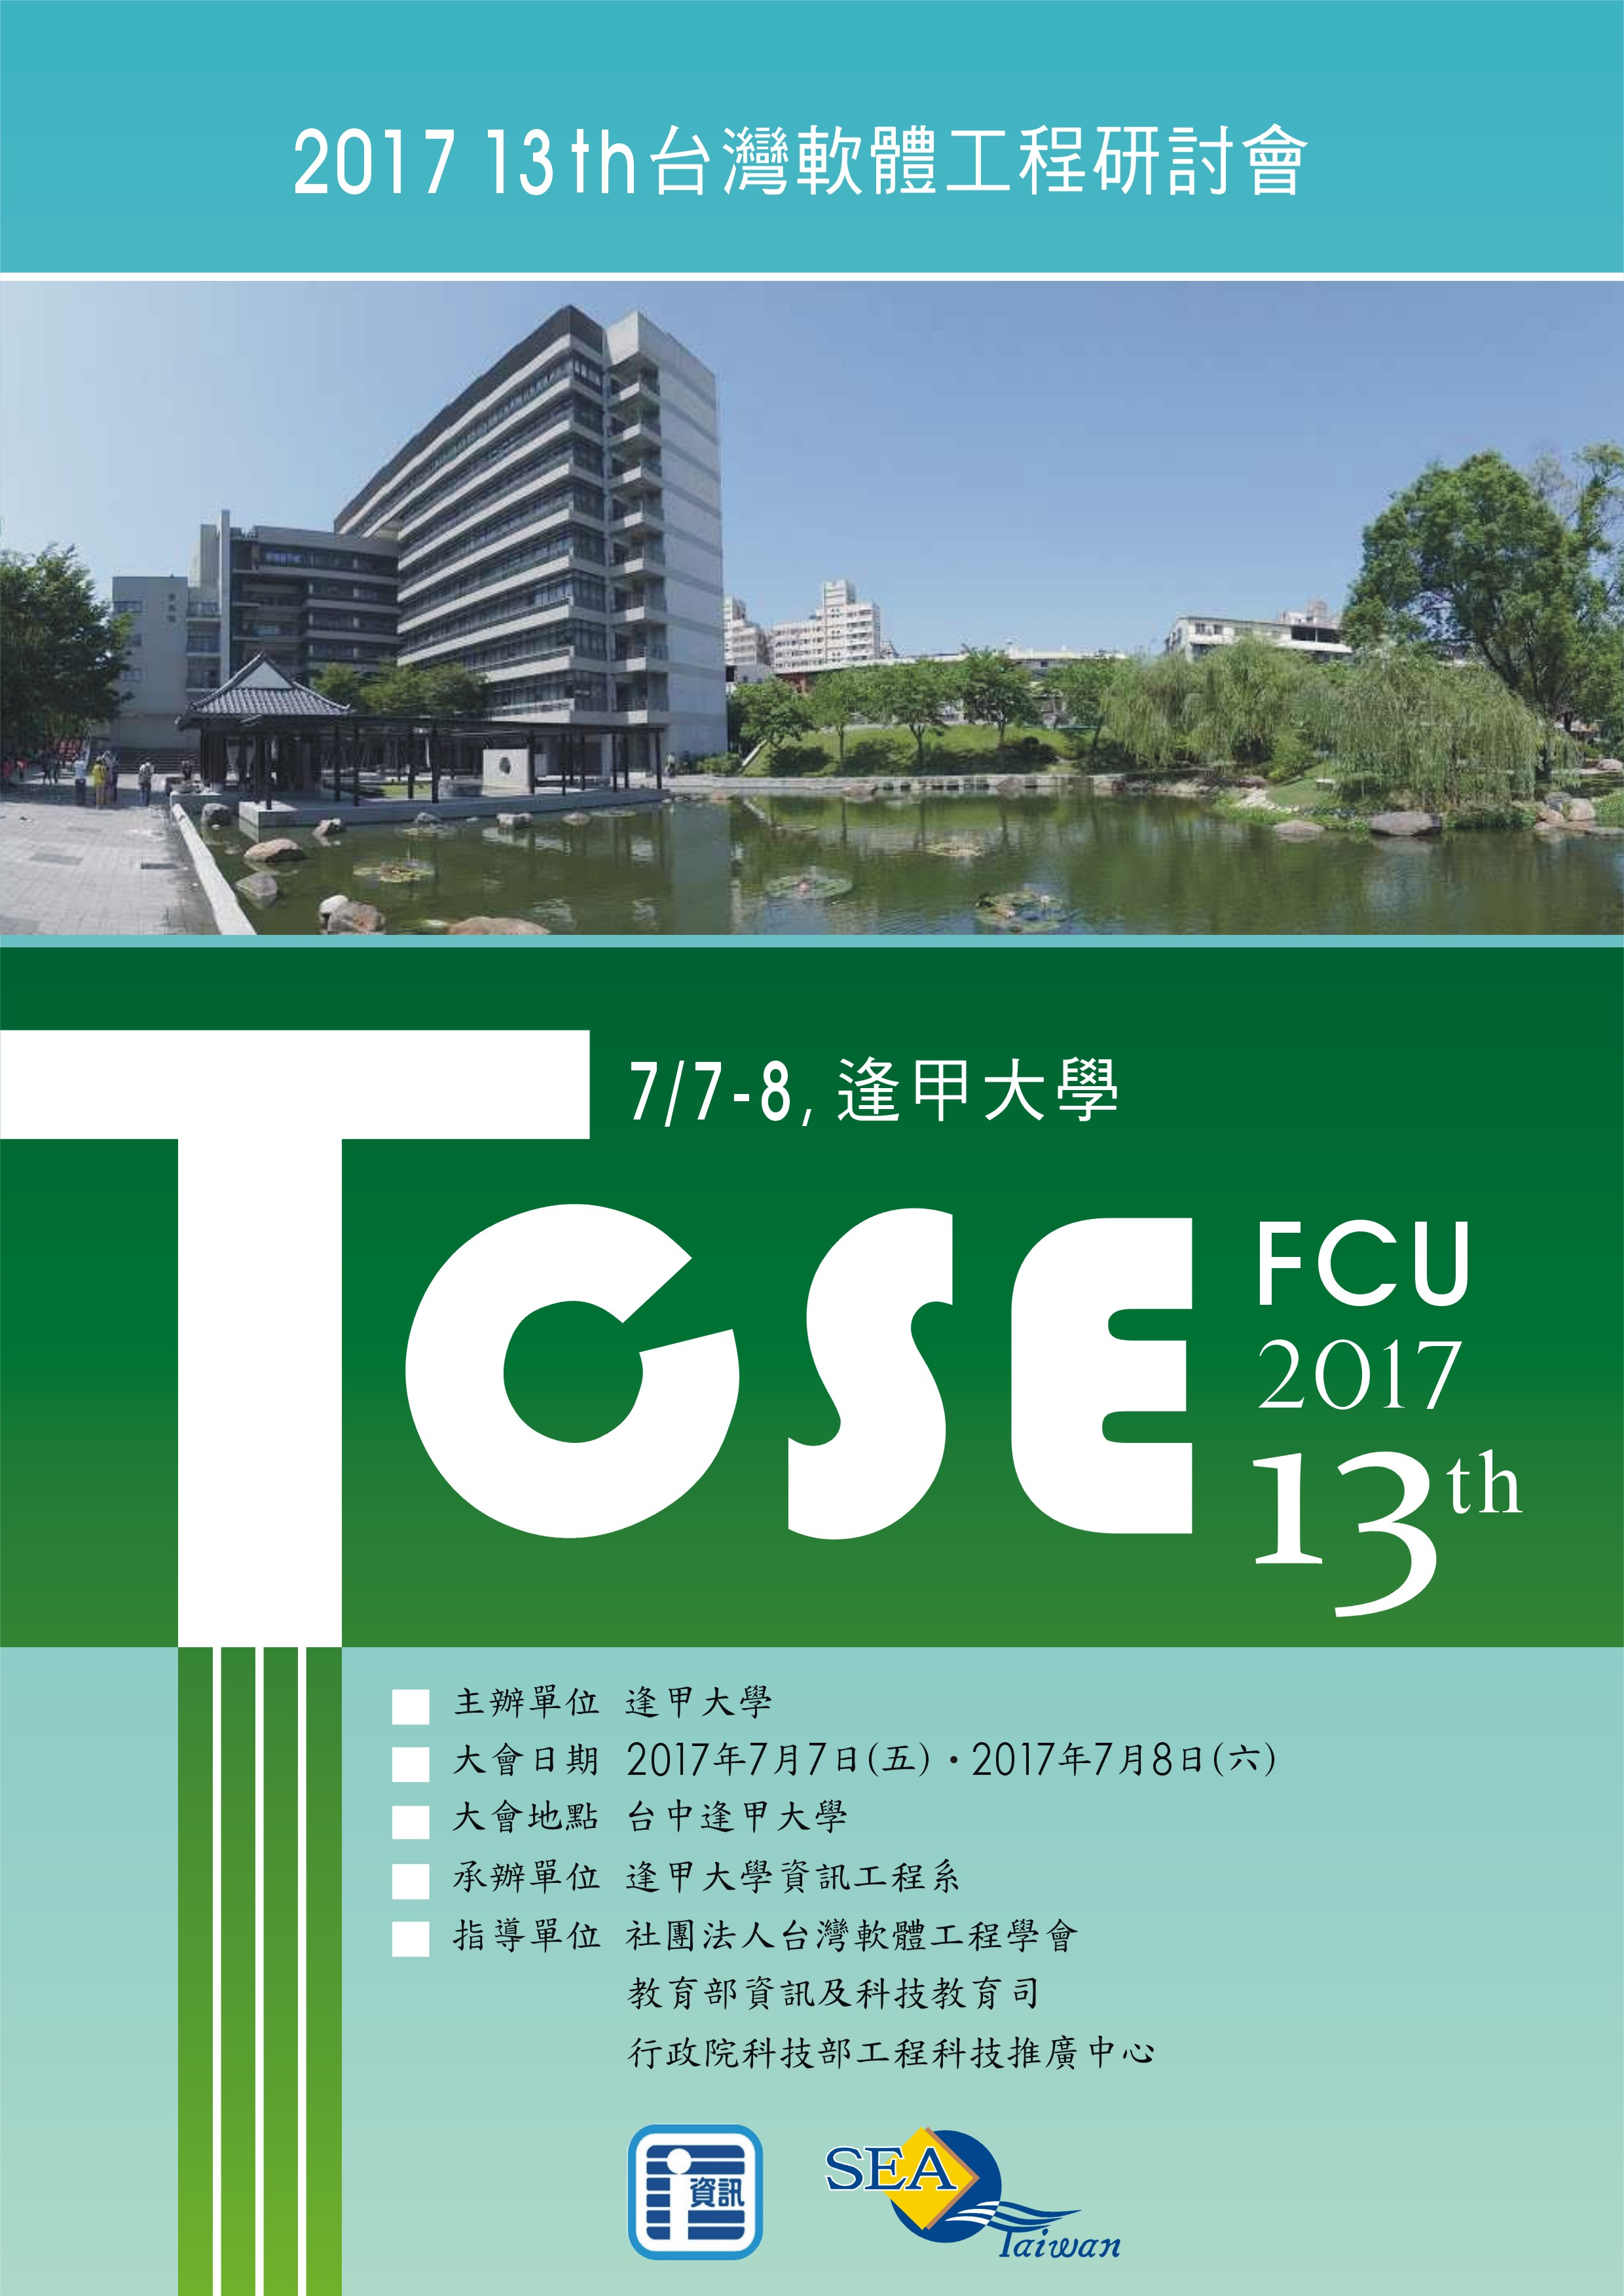
\includepdf[fitpaper]{cover} %Cover page

\chapter*{大會序言}

「台灣軟體工程研討會」(Taiwan Conference on Software Engineering, TCSE) 是台灣提供給產官學專家與學者一個探討與發表軟體工程原理、實務與最新技術 研究的園地,多年來經諸位先進積極參與,TCSE 已成為國內首屈一指的軟體相關會議。逢甲大學資工系曾經於 2007 年承辦第三屆會議,很榮幸十年後再次承辦第十三屆的研討會。

\mIndent 2017 年 TCSE 之大會主題為「\textit{Software Engineering and Data Science}」,探討軟體工程與資料科學的相關研究,包含應用軟體工程技術於資料科學及應用資料科學於軟體工程。本年度共有 83 篇投稿,最後收錄 75 篇論文,涵蓋 Software Engineering, Data Engineering, Software Testing, Web Engineering, Artificial Intelligence, Internet of Things, Software Application 等研究與實務議題。

\mIndent 今年共有兩場大會主題演講。第一天特別邀請到美國 University of Texas at Dallas 的 Prof. Lawrence Chung 主講 Big Data Analytics: A Requirements Engineering Perspective,從需求工程的角度來看資料分析。第二天邀請中研院研究員,同時也是台灣資料科學協會理事長的陳昇偉博士主講「從大數據到人工智慧」,亦是非常精采的演講。此外,今年的專題論壇(Panel Discussion),主題為 Software Engineering and Data Science,由北科大鄭有進教授擔任論壇主持人, 與談人包含台大資工李允中教授、Prof. Lawrence Chung 與帆宣系統科技韋建名副總等來自學術界與產業界的頂尖專家,透過此場合提供一個產官學界的交流平台, 共同研討軟體工程與資料科學時代之整合與應用。此外大會亦舉辦三場業界的專題演講,從實務的角度提供不同的思考視野。


\mIndent 去年的 TCSE 研討會在國立海洋大學舉辦,首次開設了 English session,鼓勵以英文撰寫並報告論文,獲得廣大迴響,優秀作品並推薦到 JIT (Journal of Internet Technology) 國際期刊刊登。今年 English paper 篇數成長至 12 篇,我們與 JISE (Journal of Information and Engineering ) 國際期刊合作,將優秀論文推薦到 JISE 的特刊。

\mIndent 為了鼓勵將軟體工程結合資料分析並鼓勵動手做,我們特別與 OpenEdu 線上學習平台及 ITSA 社群運算與巨量資料跨校資源中心合辦資料分析的黑客松競賽(Hackathon)。這也是 TCSE 首次舉辦黑客松競賽。OpenEdu 是台灣主要 MOOC (Massive Open and Online Course) 平台之一,提供優質且免費的線上課程。學習者的學習行為被完整的記錄在系統中,透過分析這些學習行為可以改善日後的線上學習方式。今年共有 6 校 13 隊 45 位同學參與初賽,通過者將於大會開始之時進行複賽,也感謝多家廠商的贊助,讓活動得以順利舉辦。

\mIndent 本次大會能順利舉辦,除了逢甲大學校方與台灣軟體工程學會的支持之外,同時也要感謝教育部資訊及科技教育司、科技部工程處工程科技推廣中心等單位的協助。對於議程主持人、議程委員、最佳論文評審所付出的精神與心力也要致上最大的感謝!此外也謝謝逢甲大學資訊工程系所有參與研討會籌備的教師以及工作人員,由於大家的群策群力才能逐步完成本次大會的規劃與目標,在此也一併致謝。最後,也敬祝 2017 年大會圓滿成功,希望與會嘉賓都能有一個愉快且有收穫的學術旅程!

\vspace{1cm}

大會主席:
\begin{tabular}{l}
許芳榮、楊東麟 
\end{tabular}

議程主席:
\begin{tabular}{l}
薛念林、陳錫民
\end{tabular}

2017 逢甲大學

% 目錄
\setcounter{tocdepth}{1} %1: section
\tableofcontents\label{toc}
\setcounter{chapter}{0}



\chapter*{大會資訊}
\addcontentsline{toc}{chapter}{\protect\numberline{} 大會資訊}%

\textbf{主辦單位} 
\begin{tabular}{l}
逢甲大學
\end{tabular}
\\

\textbf{大會日期}
\begin{tabular}{l}
2017 年 7 月 7 日(五)- 2017 年 7 月 8 日(六)
\end{tabular}
\\

\textbf{大會地點}
\begin{tabular}{l}
台中 逢甲大學\\
\end{tabular}
\\

\textbf{承辦單位}
\begin{tabular}{l}
逢甲大學 資訊工程系\\
\end{tabular}
\\

\textbf{指導單位}
\begin{tabular}{l}
社團法人台灣軟體工程學會\\
教育部資訊及科技教育司\\
行政院科技部工程科技推展中心\\
\end{tabular}
\\

\textbf{大會網站}
\begin{tabular}{l}
\href{http://tcse2017.iecs.fcu.edu.tw}{http://tcse2017.iecs.fcu.edu.tw}\\
\end{tabular}
\\

\textbf{投稿系統}
\begin{tabular}{l}
\href{https://easychair.org/conferences/?conf=tcse2017}{https://easychair.org/conferences/?conf=tcse2017}\\
\end{tabular}
\\

\textbf{社群網站}
\begin{tabular}{l}
\href{https://www.facebook.com/360848907645882/}{Facebook- 台灣軟體工程研討會} \\
\end{tabular}
\\

\textbf{聯絡方式}
\begin{tabular}{l}
信箱:mailto:tcse2017.fcu@gmail.com\\
電話:(04) 2451-7250 ext 3704\\
\end{tabular}
\\

\textbf{論文集網址}
\begin{tabular}{l}
\href{https://goo.gl/mttPFD}{https://goo.gl/mttPFD} (2017/8/31 前有效) \\
\end{tabular}
\\

\begin{figure}[h!]

\includegraphics[]{images/qr_code.png}
\end{figure}



\chapter*{大會組織}
\addcontentsline{toc}{chapter}{\protect\numberline{} 大會組織}%

\textbf{大會榮譽主席}  \\ \\
\begin{tabular}{ll}
李秉乾  & 逢甲大學校長 \\
竇其仁  & 逢甲大學資電學院院長
\end{tabular}

\textbf{大會主席} \\ \\
\begin{tabular} {ll}
許芳榮 &   逢甲大學資工系主任 \\
楊東麟 &   逢甲大學資工系教授
\end{tabular}

\textbf{議程主席} \\ \\
\begin{tabular} {ll}
薛念林 & 逢甲大學資工系 \\
陳錫民 & 逢甲大學資工系
\end{tabular}

\textbf{指導委員}\\ \\
\begin{tabular}
{p{1.8cm}p{1.8cm}p{1.8cm}p{1.8cm}p{1.8cm}p{1.8cm}p{1.8cm}p{1.8cm}}
主席:& 李允中 \\
朱正忠 &朱治平 &余孝先 & 李漢銘 &    李健興 &   周忠信 &   林哲正 &   梁德容  \\  
盛敏成 & 莊育秀 &郭耀煌 & 郭譽申 &   陳俊良  &  陳建村 &    陳英一 &   陳偉凱   \\
黃世禎 &黃為德 &   葉道明  & 劉立頌  &   劉瑞隆  &  劉龍龍 &  鄭永斌 & 鄭有進  \\  
鄭炳強
\end{tabular}
 
\textbf{特別議程主席} \\ \\
\begin{tabular}{lll}
 軟體展示:  & 李信杰 &    成功大學 資工系 \\
 企業演講: & 許懷中 &   逢甲大學 資工系 \\
 黑客松:     & 黃奕欽 &   逢甲大學 資工系 \\
 區域安排: & 徐國勛  &  台中教育大學 資工系 \\
 英文論文: & 陳奕中, 英家慶 &   逢甲大學 資工系 \\
\end{tabular}


\textbf{議程委員} \\ \\
\begin{tabular}{p{1.8cm}p{1.8cm}p{1.8cm}p{1.8cm}p{1.8cm}p{1.8cm}p{1.8cm}p{1.8cm}}
丁培毅  &  王凡  &  王建民 & 王秉豐 & 王能中 & 孔令傑&  孔崇旭 & 朱威達 \\
李文廷 & 李俊宏 &李強&  李祈鈞 &   呂學展  &  沈文祥 &   江季翰 &   吳牧恩 \\
吳秀陽 & 吳政瑋  &  吳漢銘 & 洪國鈞 & 林志敏    &林文揚 &林易泉 &林峰正 \\   
林迺衛 &林楚迪  &范姜永益 &馬尚彬 &金台齡& 孫培真& 張文貴&  張志宏    \\
張詠淳& 須上英& 梅興& 許乙清&    許子衡& 許見章 &   許煜亮& 連耀南 \\
郭忠義& 郭家旭& 童曉儒& 陳立偉&    陳炳文&    陳恭& 陳振炎&  陳伶志 \\
陳景祥& 陳宗禧& 黃冠寰& 黃建宏&    黃衍文&    黃福銘&  黃慶育&    黃惠俞\\    
黃俊穎&  楊士萱& 楊中皇& 楊豐兆&   詹大千&    賈坤芳&  廖峻鋒& 廖珗洲 \\   
熊博安& 劉豐豪& 劉建宏&  劉傳銘&    劉正山&    潘健一& 蔡敦仁& 鄭伯壎   \\ 
賴聯福& 錢炳全& 鍾毓驥&  謝仕杰&    謝孟諺&     謝政勳&    藍啟維& 羅榮華 \\
戴志華   
\end{tabular} 

\chapter*{大會議程} 


\addcontentsline{toc}{chapter}{\protect\numberline{} 大會議程}%
\begin{figure}[h!]
\begin{center}
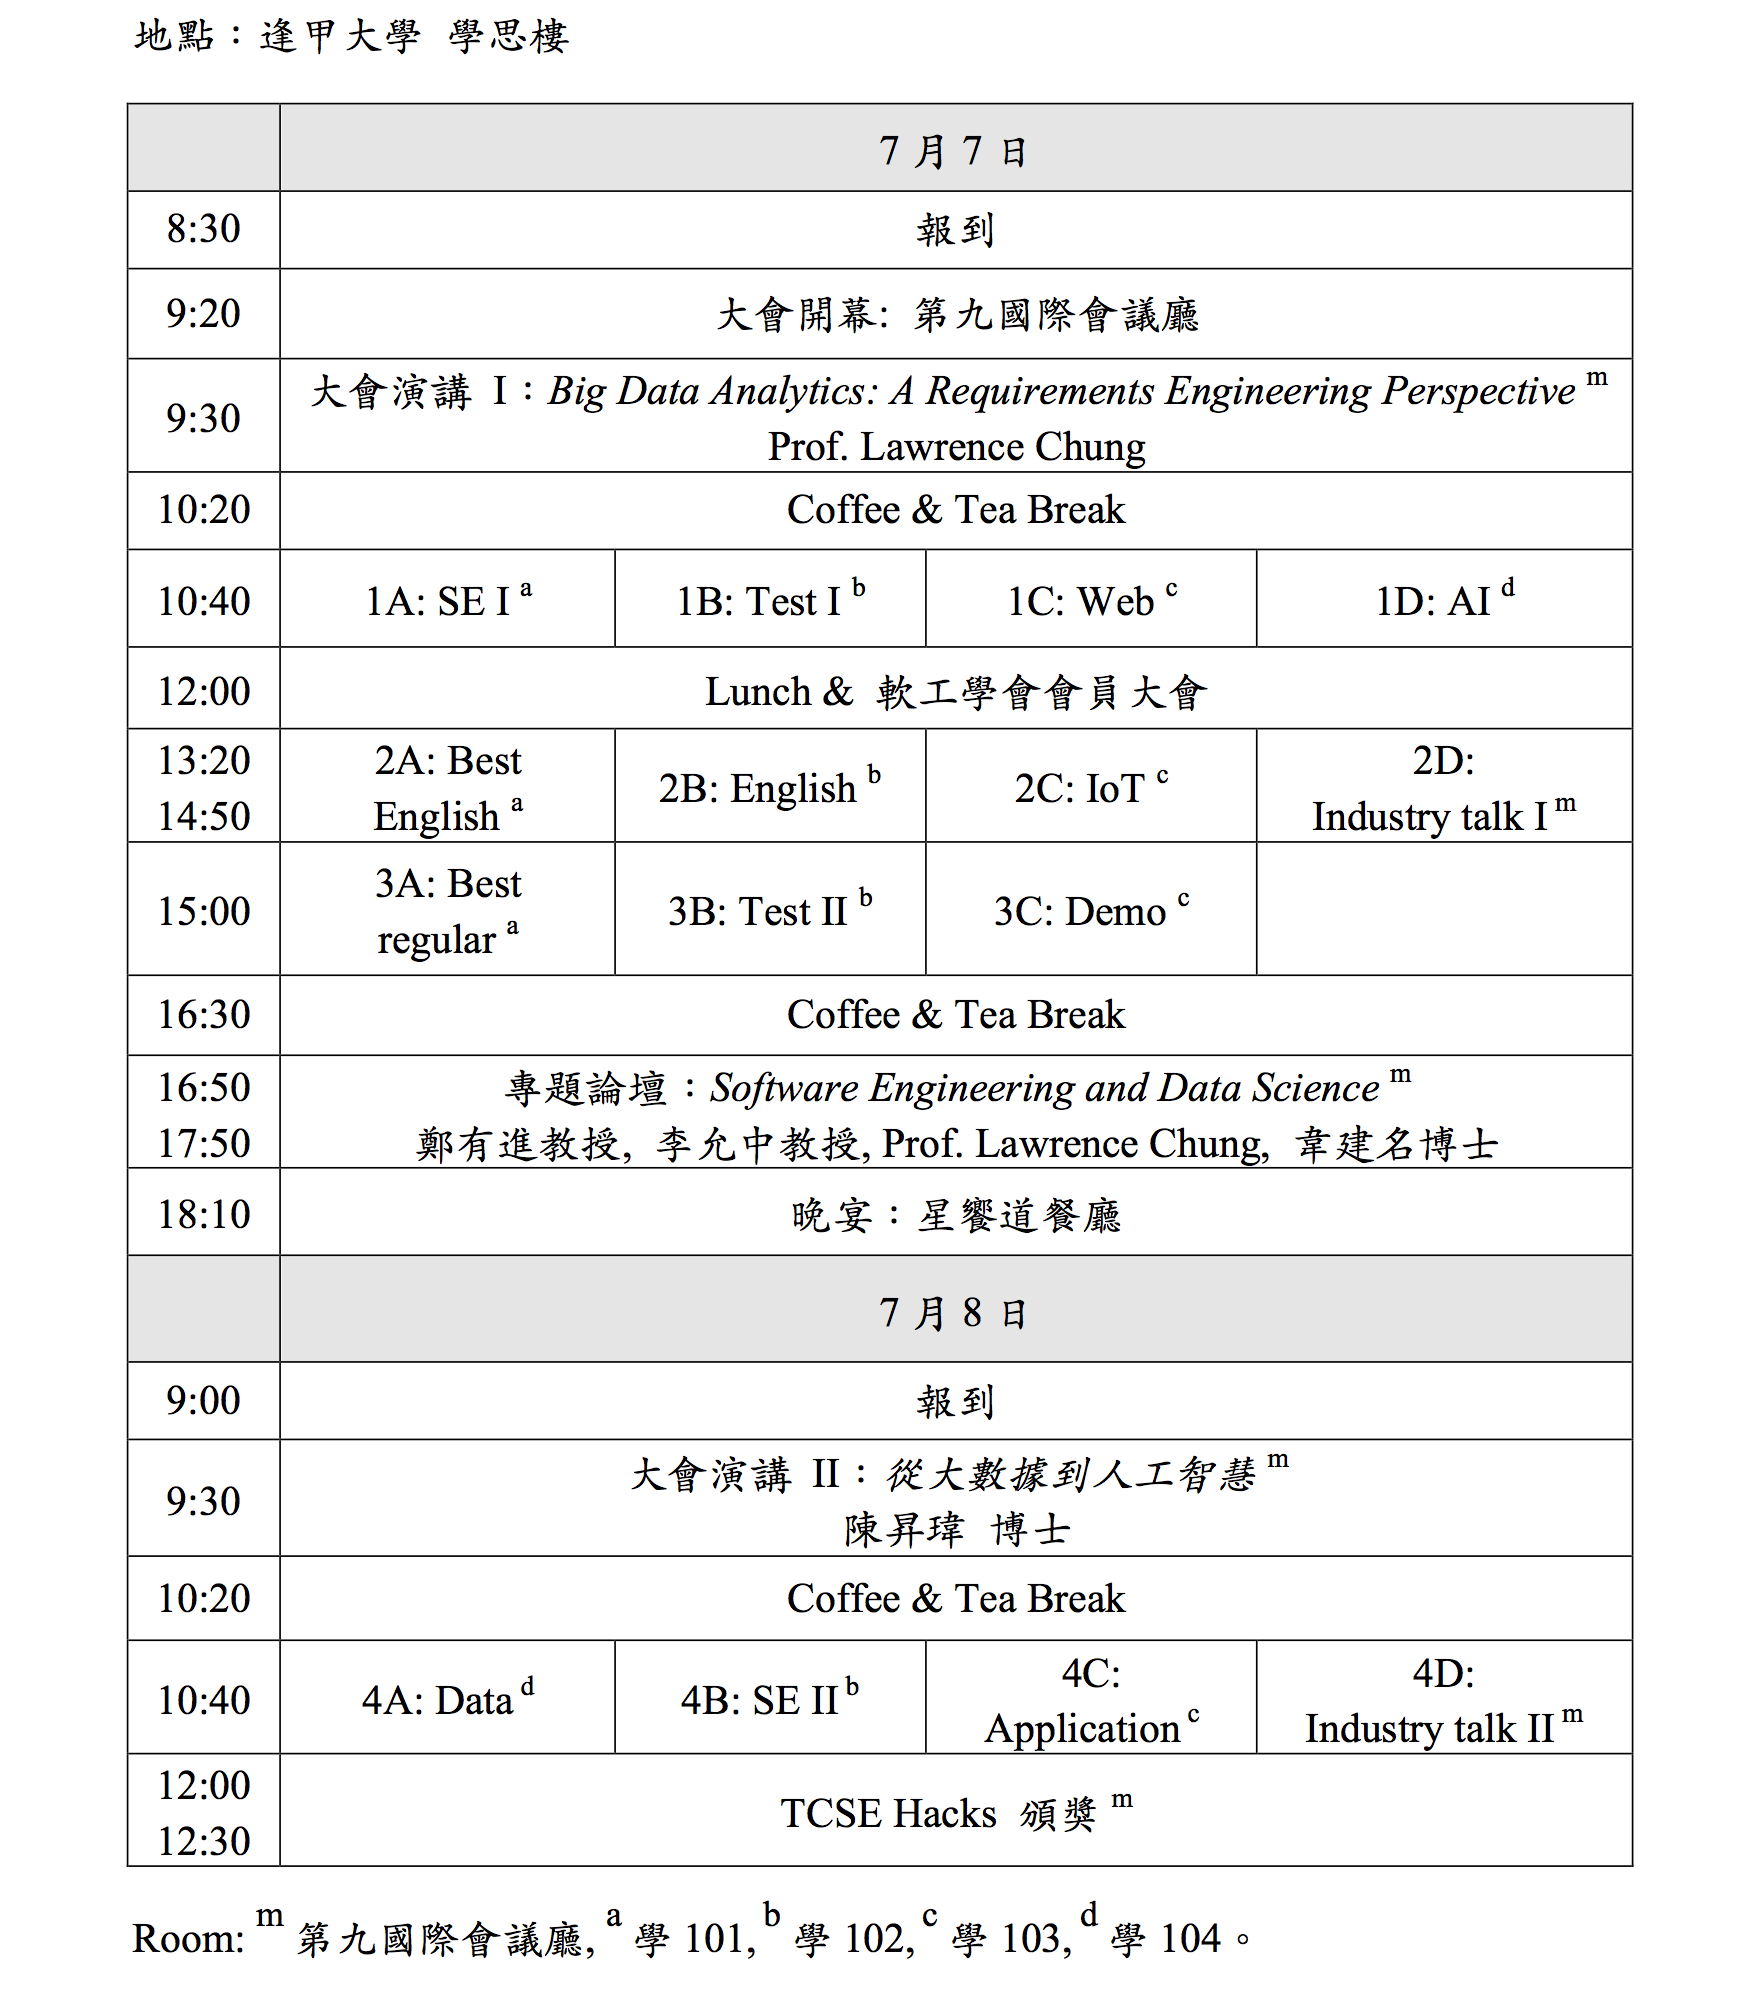
\includegraphics[width=.95\columnwidth]{images/program.png}
\end{center}
\end{figure}

\chapter*{分場詳細議程}
\addcontentsline{toc}{chapter}{\protect\numberline{} 分場詳細議程}%

\subsection*{1A: \TitleOneA}
\subsubsection*{\ChairOneA}
\ListOneA

\subsection*{1B: \TitleOneB}
\subsubsection*{\ChairOneB}
\ListOneB

\subsection*{1C: \TitleOneC}
\subsubsection*{\ChairOneC}
\ListOneC

\subsection*{1D: \TitleOneD}
\subsubsection*{\ChairOneD}
\ListOneD

\subsection*{2A: \TitleTwoA}
\subsubsection*{\ChairTwoA}
\ListTwoA

\subsection*{2B: \TitleTwoB}
\subsubsection*{\ChairTwoB}
\ListTwoB

\subsection*{2C: \TitleTwoC}
\subsubsection*{\ChairTwoC}
\ListTwoC

\subsection*{2D: \TitleTwoD}
\subsubsection*{\ChairTwoD}
\ListTwoD

\subsection*{3A: \TitleThreeA}
\subsubsection*{\ChairThreeA}
\ListThreeA

\subsection*{3B: \TitleThreeB}
\subsubsection*{\ChairThreeB}
\ListThreeB

\subsection*{3C: \TitleThreeC}
\subsubsection*{\ChairThreeC}
\ListThreeC

\subsection*{4A: \TitleFourA}
\subsubsection*{\ChairFourA}
\ListFourA

\subsection*{4B: \TitleFourB}
\subsubsection*{\ChairFourB}
\ListFourB

\subsection*{4C: \TitleFourC}
\subsubsection*{\ChairFourC}
\ListFourC

\subsection*{4D: \TitleFourD}
\subsubsection*{\ChairFourD}
\ListFourD

\chapter*{大會演講 I }
\addcontentsline{toc}{chapter}{\protect\numberline{}大會演講 I}%

\section*{Big Data Analytics: A Requirements Engineering Perspective}
\subsubsection*{\TimeKeynoteOne, \LocationKeynoteOne}

\subsection*{Prof. Lawrence Chung, Department of Computer Science University of Texas at Dallas, U.S.A.}

\begin{wrapfigure}{l}{0.3\textwidth}
%   \centering
	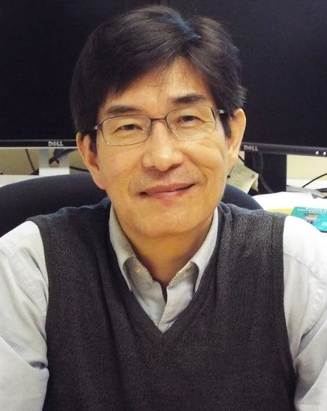
\includegraphics[width=0.3\textwidth]{images/chung.png}    
\end{wrapfigure}

Big data promises to lead to better decisions, which can bring greater operational efficiency, productivity, reduced cost and risk, and the like to a variety of domains. But is the use of big data always going to be beneficial, and if so how? In answering this question, I will first give a light survey on the use of big data in practice, along with what big data might mean. Afterwards, I will describe a goal-oriented approach to beneficially using big data. This approach is intended to rationally ``connect the dots", from stakeholders’ problems and needs, business key performance indices, important insights through analytics for both AS-IS and TO-BE, machine learning techniques, SQL/NoSQL big queries, etc. I will talk about how this approach can aid business decision making in general and more specifically in business process reengineering, possibly with a tool support. At the end, I will outline challenges in more beneficially using big data.

\paragraph{Lawrence Chung} has been working in Requirements Engineering, System/Software Architecture and Systems Engineering. He was the principal author of the research monograph “Non-Functional Requirements in Software Engineering", and has been involved in developing ``RE-Tools" (a muiti-notational requirements modeling tool kit) , ``HOPE" (a smartphone app project for people with difficulties), and ``Silverlining" (a Google-award winning project on cloud computing and big data).  He has been a keynote speaker, invited lecturer, co-editor-in-chief for Journal of Innovative Software, editorial board member for Requirements Engineering Journal and  International Journal of Networked and Distributed Computing, editor for ETRI Journal, and program co-chair for various international events.  He is currently on the faculty of Computer Science at University of Texas at Dallas.  He received his Ph.D. in Computer Science in 1993 from University of Toronto.

\chapter*{大會演講 II}
\addcontentsline{toc}{chapter}{\protect\numberline{}大會演講 II}%

\section*{從大數據到人工智慧}
\subsubsection*{\TimeKeynoteTwo, \LocationKeynoteTwo}


\subsection*{陳昇瑋 博士,台灣資料科學協會理事長}

\begin{wrapfigure}{l}{0.3\textwidth}
	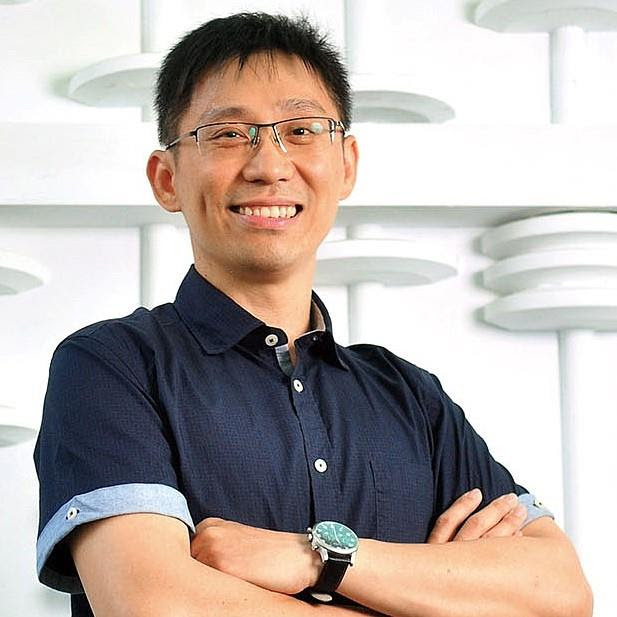
\includegraphics[width=0.3\textwidth]{images/chen.jpg}    
\end{wrapfigure}

大數據在台灣蔚為風潮,無論是政府官員或販夫走卒,人人皆聽聞大數據的威力。因此,產業界及各級政府皆努力建置所謂的大數據平台,以蒐羅及保存資料為己任,並導入資料的視覺分析工具,讓決策者們能夠快速地查看管理或施政成效,以客觀數據來輔助主觀評價,以分析輔助經驗,以事實取代臆測。

\mIndent 這些都是好的進展。收集資料並整理成視覺化的分析圖表,對於評估及掌控現況有非常大的幫助,讓我們不再只能依直覺及經驗做決策。但,其實,這只是把資料平台準備好而已,要充份發揮資料的價值,還沒有沾到邊。要發揮資料價值,不能光談大數據,機器學習與人工智慧是絕對不該忽略的。事實上,這三者環環相扣:大數據是材料,機器學習是處理方法,人工智慧是成品所呈現的特質。這個時代,蒐集了大量資料,只呈現給人看,而不是拿來餵給電腦學習,讓你的應用呈現人工智慧,就跟採集了大量松露結果拿來沾醬油一整碗吃掉一樣可惜。如同精靈寶可夢需要有訓練師才能發揮能力,擁有大數據後,我們也需要很多很多的機器學習專家(有人稱呼為AI訓練師),才能讓我們手中的大數據真正發揮價值。

\mIndent 在此演講中,我將為聽眾闡明資料科學、大數據、人工智慧、機器(深度)學習、資料探勘等相近但又不同的詞彙,再以各領域的實際案例來分享資料的可能應用及實用價值。同時,我將與聽眾分享其協助多家企業培訓資料科學家及導入資料科學團隊的各種經驗,從企業如何跳脫既有框架,讓資料科學團隊盡情揮灑無限創意著手,進而能活用資料、挖掘出潛藏在資料中不為人知的秘密,最終打造高信任度及高效率的工作環境,展現資料分析的價值。

\paragraph{陳昇瑋博士} 現為台灣資料科學協會理事長、中央研究院資訊科學研究所研究員暨資料洞察實驗室主持人,研究領域為大數據分析、深度學習、計算社會科學及多媒體系統等,在使用者/社群意見及感受的淬取及量化方面持續有代表性的研究創見。陳博士堅信資料及資料分析的價值,長期推廣資料科學及其在各領域的應用,發起台灣資料科學協會及台灣資料科學年會,期能將對於資料科學的熱情傳達給大眾,一起來探索資料科學的潛力,並將資料科學引入每個人的專業領域之中。他期待讓資料分析在台灣不再是口號,而是大家真實拿來解決問題及創造價值的工具。更多資訊可參考其\href{http://www.iis.sinica.edu.tw/~swc/index_c.html}{個人網頁}。

\chapter*{專題論壇}
\addcontentsline{toc}{chapter}{\protect\numberline{}專題論壇}%

\begin{figure}[h!]
\begin{center}
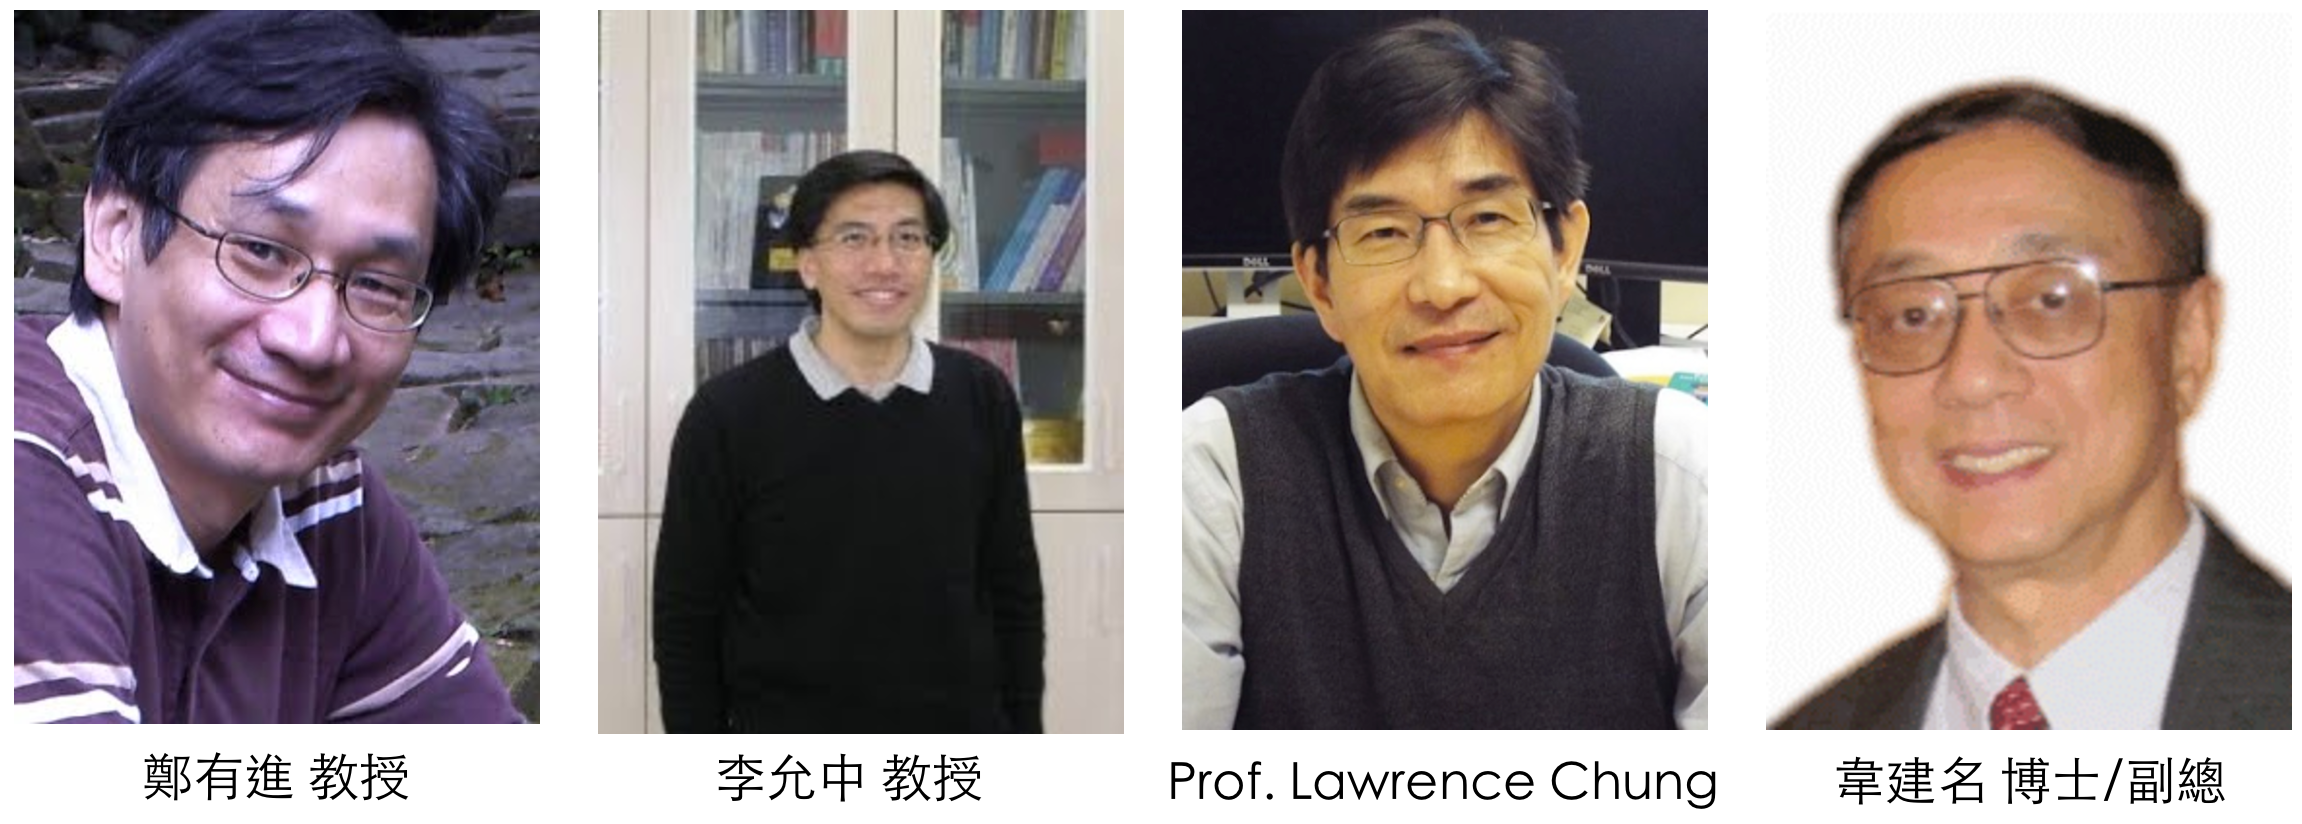
\includegraphics[width=1\columnwidth]{images/panel.png}
\end{center}
\end{figure}

\section*{Topic: Software Engineering and Data Science}

\subsubsection*{\TimePanel, \LocationPanel}

\subsubsection*{主席:鄭有進教授 / 國立臺北科技大學}

\mIndent 鄭有進教授任職於台北科技大學資工系,教授物件導向程式設計、樣式導向設計、軟體架構、軟體需求與規格、人工智慧等課程。最近,他為大學生學習物件導向程式設計寫了中文部落格How To Solve It – OOP (http://htsioop.blogspot.tw/)與英文部落格How To Solve It – CPP (http://htsicpp.blogspot.tw/)。他於2009/12~2012/11三年間主持學界科專計畫,致力於推廣敏捷方法Scrum,協助多家台灣的資通訊廠商改善其軟體專案的開發效率與品質;該科專計畫並產出自由軟體ezScrum (http://sourceforge.net/projects/ezscrum/)供全球社群使用。鄭教授現曾任台灣軟體工程學會秘書長、理事長,他也是IEEE Computer Society的會員,並於2010年獲得Scrum Alliance的Certified ScrumMaster資格。鄭教授畢業於台北工專 (1985),隨後獲得美國Johns Hopkins University碩士學位(1990)與University of Oklahoma博士學位(1993)。



\subsubsection*{與談人:李允中教授 / 國立臺灣大學資訊工程系}
\begin{tabular}{ll}
學 歷: & Computer Science 博士,Texas A\&M University\\
現 職: & 教授,國立台灣大學 資訊工程學系 \\
經 歷: & 技術顧問,經濟部技術處 \\
   & External Examiner UNITEN, Malaysia \\
   & 理事長, 台灣軟體工程學會 副主席 國際模糊學會(IFSA) \\
   & 召集人, 經濟部技術處 SBIR資通領域 \\
   & 召集人, 教育部顧問室 軟體工程聯盟 \\
   & 教授, 國立中央大學 資訊工程學系  \\
   & 主任, 國立中央大學 電子計算機中心 \\ 
   & 系主任, 國立   中央大學 資訊工程學系 \\
獲 獎: & IBM 全球聯合大學研究(SUR)獎助 \\ 
   & 傑出電機工程教授, 中國電機工程師學會 \\
   & 特聘教授, 國立中央大學 
\end{tabular}

\subsubsection{與談人:Prof. Lawrence Chung / Department of Computer Science, University of Texas at Dallas}

\mIndent Lawrence Chung has been working in Requirements Engineering, System/Software Architecture and Systems Engineering. He was the principal author of the research monograph ``Non-Functional Requirements in Software Engineering", and has been involved in developing ``RE-Tools" (a muiti-notational requirements modeling tool kit) , ``HOPE" (a smartphone app project for people with difficulties), and ``Silverlining" (a Google-award winning project on cloud computing and big data).  He has been a keynote speaker, invited lecturer, co-editor-in-chief for Journal of Innovative Software, editorial board member for Requirements Engineering Journal and  International Journal of Networked and Distributed Computing, editor for ETRI Journal, and program co-chair for various international events.  He is currently on the faculty of Computer Science at University of Texas at Dallas.  He received his Ph.D. in Computer Science in 1993 from University of Toronto.


\subsubsection*{與談人:韋建名 博士 / 帆宣系統科技股份有限公司}

\mIndent 韋博士在電腦,通信,網路及軟體產業界已有超過40年以上的經驗。過去曾服務於IBM、貝爾實驗室(Bell Laboratories)、Racal-Milgo、Fibronics/Spartacus、Axonet、瑞博强芯(天津)科技有限公司及目前的帆宣系統科技股份有限公司。他所負責的工作範圍涵蓋了策略規劃、系統架構設計、產品研發銷售、技術管理與行政管理等事務。他曾有五次創業及公司轉型的成功經驗,並成功地研發及推出超過20種以上的商業產品。

\mIndent 韋博士從美國康州大學(University of Connecticut)工學院,電機及計算機科學系 (Electrical Engineering and Computer Science Department)獲得他的學士(1971)、碩士(1973)及哲學博士(1978)學位。他也是美國康州大學工學院1995年的 ``傑出工程師校友獎”的得獎人。

\chapter*{企業演講}
\addcontentsline{toc}{chapter}{\protect\numberline{}企業演講}%


%\begin{figure}[h!]
%\begin{center}
%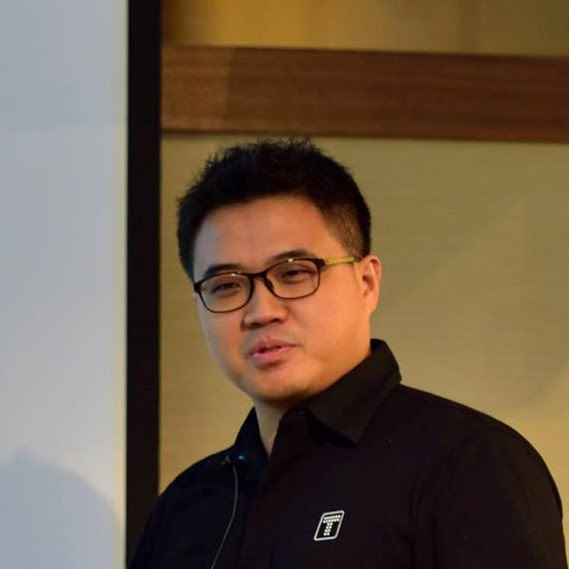
\includegraphics[width=.2\columnwidth]{images/yves.yves}
%\end{center}
%\end{figure}

\section*{空手、緊握、到放手 – 敏捷路上學到的5件事} 
\subsection*{林裕丞 總經理 / 新加坡鈦坦科技} 
\subsubsection*{\TimeIndustryOne, \LocationIndustryOne}

\begin{tabular}{l m{12cm}}
	\begin{minipage}{4.5cm}
		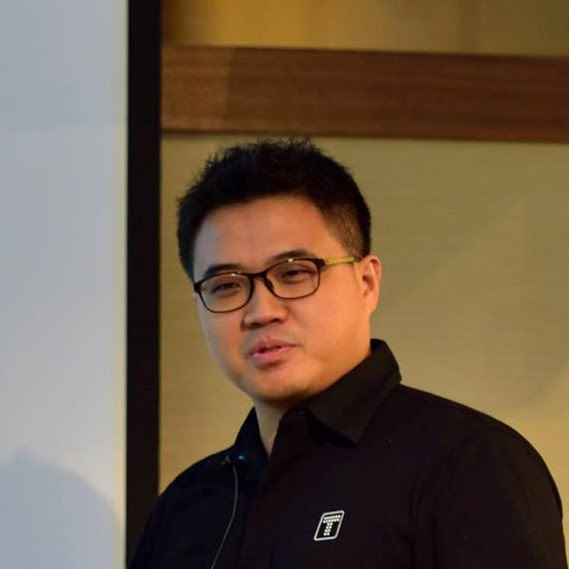
\includegraphics[width=4.2cm]{images/yves.jpg}   
    \end{minipage}
	&    
	為什麼吃飽沒事做要跑敏捷?從一開始新加坡5人,到現在跨國150人,這過程中有喜悅、有掙扎、也有不少的學習和成長。這是一個鈦坦科技十年來的演化史,經由長時間跨度與宏觀組織角度,跟大家分享我們在組織文化和產品面上的改變和學習。在這次演講中您將會有以下收穫:
\begin{enumerate}
\item 什麼時候要跑敏捷?
\item 如何評估敏捷的成效?
\item 在組織管理上有那些工具和方法?
\end{enumerate} 
\end{tabular}

\section*{協同式雲端作業系統 - 創造雲端社會的新生態} 
\subsection*{林俊孝 Chief Technology Officer/ Picowork} 
\subsubsection*{\TimeIndustryTwo, \LocationIndustryTwo}


\begin{tabular}{l m{12cm}}
	\begin{minipage}{4.5cm}
		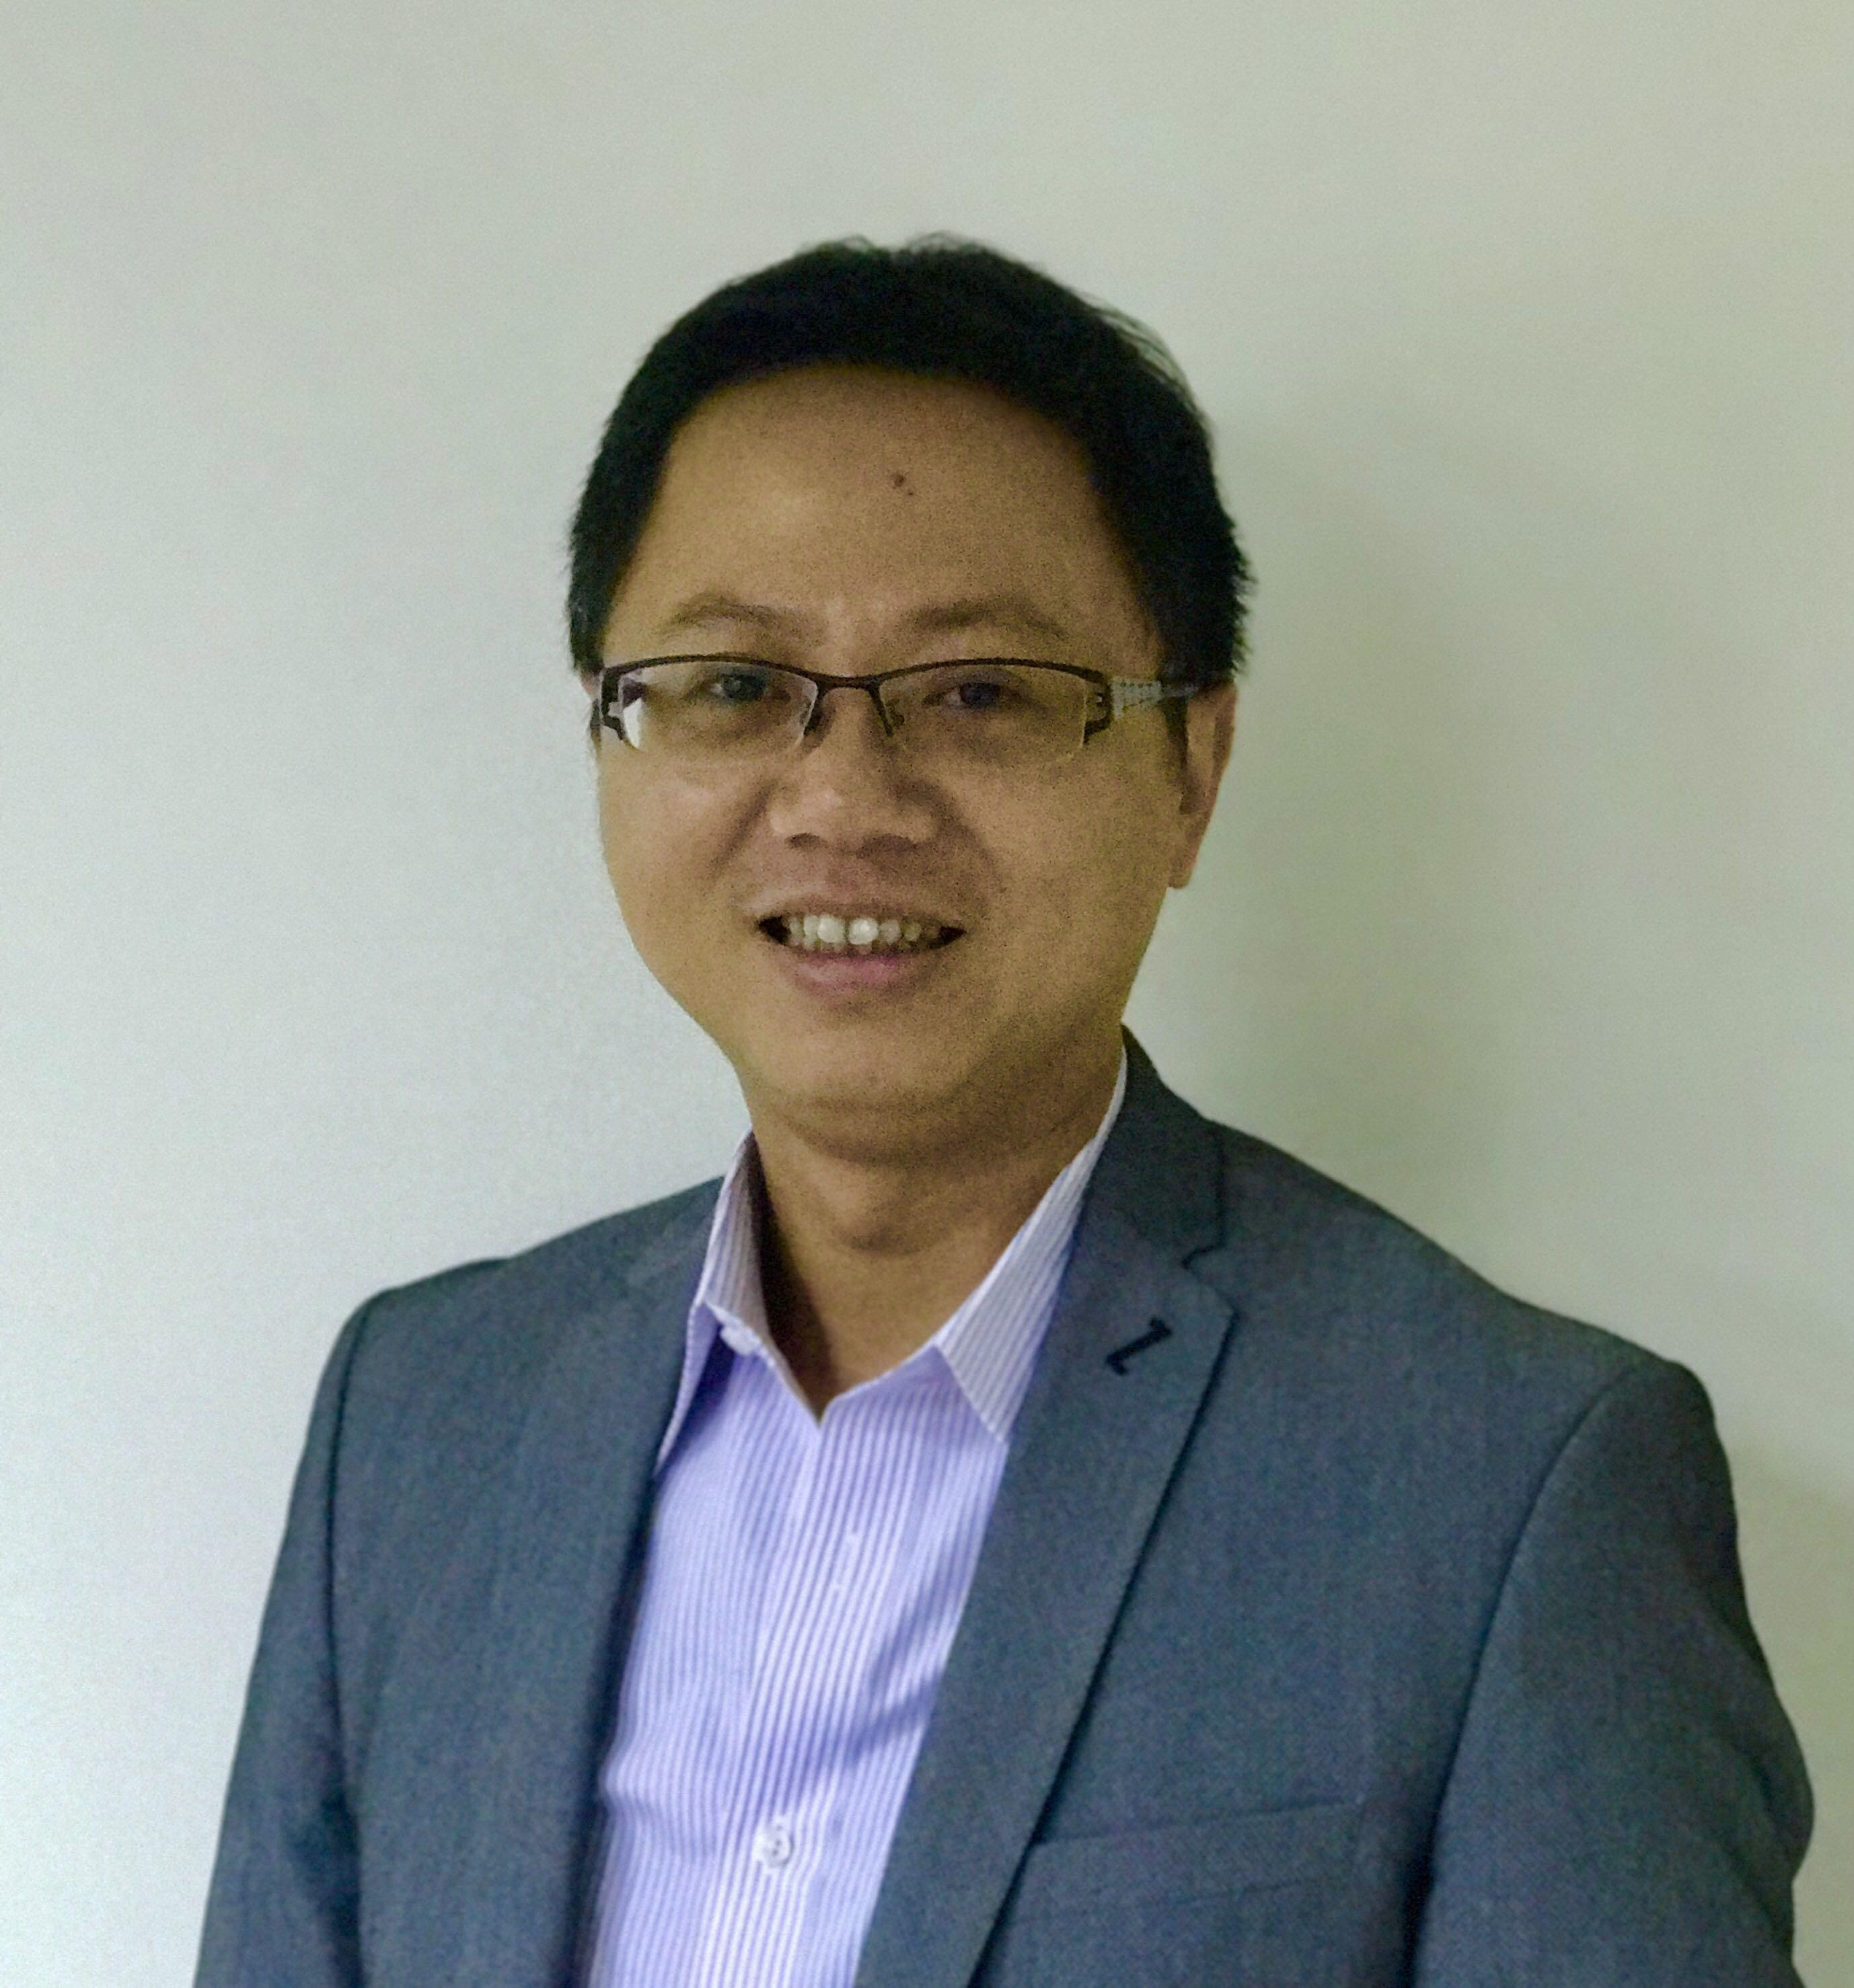
\includegraphics[width=4.2cm]{images/lin.jpeg}    
    \end{minipage}
	&    
現今的生活大量的依賴第三方應用服務來進行,然而不同的應用服務和服務平台間存在著商業經營上、技術架構上、及功能發展上及壁壘(Boundry),帶來產業全方位協同的挑戰。「協同式雲端作業系統」以作業系統的角度出發,透過技術思維上的創新,將整個網際網路看成是全球最大的一部計算機,重新定義了網際網路的定位,使各行各業可以擁有自己的雲端作業系統環境,又可以透過自己的雲端環境,與任何人(同事、顧客、夥伴、朋友)自由地進行協同作業,也能以最低的成本,讓過去、現在、及未來的網路資訊系統和網路資源擴充到雲端環境中,最後亦能藉此產生自我的大數據,為創造雲端社會的新生態,帶來了新的可能。
\end{tabular}

\clearpage

\section*{資料科學在物聯網之應用} 
\subsection*{王燚 / MathWorks財務工程技術經理}
\subsubsection*{\TimeIndustryThree, \LocationIndustryThree}

\begin{tabular}{l m{12cm}}
	\begin{minipage}{4.5cm}
		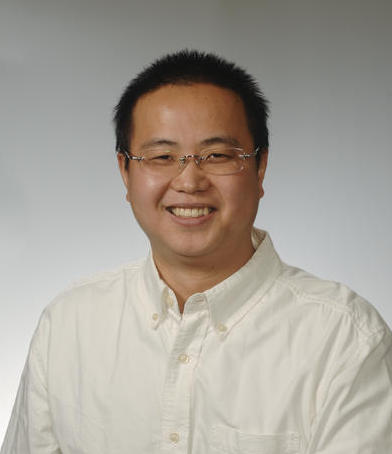
\includegraphics[width=4.2cm]{images/YiWang.jpg}    
    \end{minipage}
	&
	使用資料科學技巧將龐大複雜的資料轉化成可使用的資訊已經變成炙手可熱的趨勢,因為它能夠協助提升工程設計及決策流程的效率。不過,目前資料科學最大的挑戰,在於如何發展出有效的解析(analytics)結果,並將其整合到生產系統如無論是企業使用的 Hadoop、Spark、Tableau 或各種資料庫,甚至是各式各樣嵌入式感測器所構成的物聯網 (IoT) 環境中等等。本演講將介 MATLAB針對這些挑戰所提出的解決方法和技術,對於那些從未聽說過 MATLAB 的您來說,將會體會到為何 MATLAB 為何會成為全球工程師和科學家進行研發工作的關鍵性分析和建模的高效平台;而對已經是 MATLAB 的使用者來說,本演講也將讓您了解 MATLAB 的最新功能,如何協助您進一步簡化並加速完成您的資料科學任務。
	
%王經理專精領域為金融建模、生產導入整合以及MATLAB平行計算。目前,王燚爲金融服務機構和壽險相關MATLAB用戶提供服務,協助建構穩健且功能齊全的金融模型,以便提升工作效率。他也爲美國聯邦儲備銀行、美國聯邦儲備委員會以及其他代表性的商業銀行和對沖基金機構講授MATLAB講座和實機操作課程。王經理擁有多倫多大學計算機工程應用科學學士學位,南加州大學計算機科學碩士學位,2007年加入MathWorks之前,他在伊利諾伊州摩托羅拉工作了七年,從事無線通訊産品的軟體開發。目前於哈佛大學在職進修金融相關課程、並通過了加拿大證券課程考試及CFA二級考試。

\end{tabular}


\chapter*{JISE Special Issue}
\addcontentsline{toc}{chapter}{\protect\numberline{}JISE Special Issue}%

\section*{Special Issue on Interdisciplinary Study on 
Software Engineering and Data Science}

投稿 TCSE English Session, 並獲選為 Best paper 者,將推薦至此 Special Issue。

\mIndent Data science is a cross-domain research field which integrates information technologies and statistical methods to extract knowledge and insights from various kinds of data. Along with the maturity of big data techniques and infrastructures, a huge amount of data can now be collected, stored, and processed for further exploration of hidden information and values. Recommendation systems, internet of things, and applications adopting machine learning and deep learning etc. are all developed on the basis of the rapid growth of data science. 

\mIndent However, the development of a data system, an information technology system working together with data deluge, is now still more an art than an engineering process. Conventional software engineering methods do not suit the development of a data system. For example, the capability of a data set, e.g., what a data set can be adopted for, cannot be revealed without data discovery. In other words, the requirements of a data system are gradually discovered during system development. The bugs within a data system which corrupt the data may dramatically influence the performance of a data system without generating any faulty behavior. Since data and data science techniques would play an essential role for future information systems, studies of software engineering methods and tools on the development of data systems can be essential. 

\mIndent On the other hand, the statistical data generated from conventional software engineering methods can also be used on improving the methods. Developing and running software generates a large amount of data about the software engineering process and the user usage, which can become useful information with the help of data science. Mining design patterns and performance impact factors are two interesting examples. Adopting data analytics techniques on software engineering becomes an important issue for software engineering study in software development life cycle.

\paragraph{Scopes} The special issue welcomes the original contribution that addresses (1) the software engineering methods for data systems/products and data techniques, and (2) the data analytics techniques for software engineering methods.

\begin{itemize}
\item Utilities and environments for data engineering, analytics, and applications
\item Software engineering for big data infrastructure 
\item Software engineering for data systems/products
\item Software engineering for IoT 
\item Software engineering for data processing and engineering
\item Inductive software engineering 
\item Data mining on software engineering repositories
\item Data analytics for software engineering 
\item Validation and Verification of data systems/products
\item Systematic methods for data de-identification 
\end{itemize}

\paragraph{Author’s Guidelines} The submission should follow the formatting guidelines of the Journal of Information Science and Engineering (http://jise.iis.sinica.edu.tw/pages/authors/index.html). Any questions regarding this special issue should be sent to the guest editors. All submitted papers will be reviewed by at least three reviewers and selected based on their originality, significance, relevance, and clarity of presentation. Prospective authors should submit full manuscripts with PDF format electronically to http://journal.iis.sinica.edu.tw/url/jise-seds by 8/30/2017.

\paragraph{Publication Schedule}
\begin{itemize}
\item Manuscript submission deadline: 8/30/2017
\item Notification of Acceptance/Rejection/Revision: 11/30/2017
\item Final Manuscript Due: 12/31/2017
\item Tentative Publication Date: 2018
\item For more information, please contact the guest editors.
\end{itemize}

\textbf{Guest editors:}
\begin{itemize}
\item Yu-Chin Cheng, National Taipei University of Technology, Taiwan, yccheng@csie.ntut.edu.tw
\item Ji Zhang, The University of Southern Queensland, Australia, Ji.Zhang@usq.edu.au
\item Chang-Shing Lee, National University of Tainan
Taiwan, leecs@mail.nutn.edu.tw
\item Don-Lin Yang, Feng Chia University, Taiwan, dlyang@fcu.edu.tw
\end{itemize}

\chapter*{TCSE Hacks 黑客松競賽}
\addcontentsline{toc}{chapter}{\protect\numberline{}TCSE Hacks 黑客松}%

\begin{figure}[h!]
\begin{center}

\includegraphics[width=1\columnwidth]{images/Hackathon_logo1.png}
\end{center}
\end{figure}

TCSE 2017大會的主題為「Software Engineering and Data Science」,將探討軟體工程與資料科學的相關研究,包含應用軟體工程技術於資料科學及應用資料科學於軟體工程。為了推廣軟體工程與資料科學的整合應用,特舉辦此競賽。

\mIndent 今年我們將以 MOOCs (Massive Open Online Courses) 線上學習系統的資料為分析對象。OpenEdu 是台灣主要 MOOCs 平台之一,提供優質且免費的線上學習課程。學習者的學習行為被完整的記錄在系統中,透過分析這些學習行為可以改善日後的線上學習方式。本黑客松的活動希望大家能夠應用程式及資料分析的技巧,挖掘及了解學生值得探討的學習行為模式。

\mIndent 用於競賽的資料包含去識別化後,共約 80 門 OpenEdu 線上課程之學生登出入、觀看影片、回答線上問題、留言板討論等紀錄。而我們的最終目的是,希望參賽各組可以透過這些資料建立期初表現與期末表現的預估模型。因此在黑客松複賽前,我們將提供修習記錄等資料供參賽隊伍進行資料清理與理解的相關工作,而比賽當天主辦方將提供其中約 56 門課學生的期末表現,作為訓練資料集的標籤,然後使用餘下約 24 門課學生的期末表現結果,作為測試資料標籤。

\mIndent 各組所建構之模型在測試資料集上的表現(如準確率、召回率等) 為競賽評分的主要依據,此外,為了鼓勵參賽隊伍使用軟體工程方法,主辦單位也將於黑客松進行過程中觀察各組的工作狀況,作為軟體工程實務獎項的評分依據。

重要日期

\begin{itemize}
\item MATLAB 工作坊:5/31
\item 初賽報名截止:6/1
\item 初賽:6/2-6/15
\item 複賽:7/7-7/8, 逢甲大學
\end{itemize}

\begin{bottompar}
活動協辦:ITSA社群運算與巨量資料跨校資源中心,OpenEdu, 逢甲大學大數據中心 \\
活動贊助:鈦坦科技,鈦思科技,Picowork, 資拓宏宇, 誠雲科技, 台灣軟體工程學會
\end{bottompar}

\begin{comment}
\section*{參賽辦法}

\begin{itemize}
\item 需為在校學生組隊參加,每組 2-4 人,需有一位學校教師推薦或領隊。

\item 初賽:
	\begin{itemize}
	\item 6/1  (四) 前報名,每組 2-4 名為限。
	\item 6/2(五)上午10:00 初賽題目公布在網路,回傳結果必須正確,依回覆速度排名,最多取十名進入複賽,於 6/15 日公布於網站。	
	\end{itemize}

\item 複賽:
	\begin{itemize}
	\item 	外縣市(非台中市區)支隊伍,大會補助 2,000 住宿費。
	7/7-7/8 於逢甲大學 TCSE 2017會場報到後進行複賽。
	7/8 上午10:30-12:00 各組報告,選出名次。
	\end{itemize}

\item 設備:
	\begin{itemize}
	\item 研討會提供電腦教室、電腦網路、無線網路,可自行帶電腦。
評分標準
	\item 精準度:預估的精準度。
	\item 軟體工程實務:開發過程中是否發揮團隊合作精神,及相關的軟體工程實務做法,例如開發方法論,設計方法,測試方法等。此項目的評分來自:(1) 過程中委員的觀察 (2) 最終報告時團隊的簡報。
	\end{itemize}
\end{itemize}

\end{itemize}
 
\section*{獎金}
\begin{itemize}
\item 第一名:新台幣 15,000(1 名)
\item 鈦坦科技軟體工程實務特別獎:新台幣 8,000(1 名)
\item MATLAB 特別獎:新台幣  5,000(1 名)
\item 黑客松精神獎:3,000 (1-5 名)
\item 一組僅能獲得一個獎項。
\end{itemize}

\end{comment}

\ifShowPaper
\chapter{Software Engineering, Software Testing, Web Engineering and AI}

\TimeOne

\section{\TitleOneA}
\subsection*{\ChairOneA}
\ListOneA
\PaperOneA

\section{\TitleOneB}
\subsection*{\ChairOneB}
\ListOneB
\PaperOneB

\section{\TitleOneC}
\subsection*{\ChairOneC}
\ListOneC
\PaperOneC

\section{\TitleOneD}
\subsection*{\ChairOneD}
\ListOneD
\PaperOneD

\chapter{English paper, IoT and Industry Talk I}
\TimeTwo

\section{\TitleTwoA}
\subsection*{\ChairTwoA}
\ListTwoA
\PaperTwoA

\section{\TitleTwoB}
\subsection*{\ChairTwoB}
\ListTwoB
\PaperTwoB

\section{\TitleTwoC}
\subsection*{\ChairTwoC}
\ListTwoC
\PaperTwoC

\section{\TitleTwoD}
\subsection*{\ChairTwoD}
\ListTwoD

\subsection*{題目:空手、緊握、到放手 – 敏捷路上學到的5件事}

\subsubsection*{演講者:林裕丞 總經理 / 新加坡鈦坦科技}

為什麼吃飽沒事做要跑敏捷?從一開始新加坡5人,到現在跨國150人,這過程中有喜悅、有掙扎、也有不少的學習和成長。這是一個鈦坦科技十年來的演化史,經由長時間跨度與宏觀組織角度,跟大家分享我們在組織文化和產品面上的改變和學習。在這次演講中您將會有以下收穫:(1) 什麼時候要跑敏捷?(2) 如何評估敏捷的成效?(3) 在組織管理上有那些工具和方法? 


\subsection*{題目:協同式雲端作業系統 - 創造雲端社會的新生態}

\subsubsection*{演講者:林俊孝 Chief Technology Officer/ Picowork}

現今的生活大量的依賴第三方應用服務來進行,然而不同的應用服務和服務平台間存在著商業經營上、技術架構上、及功能發展上及壁壘(Boundry),帶來產業全方位協同的挑戰。「協同式雲端作業系統」以作業系統的角度出發,透過技術思維上的創新,將整個網際網路看成是全球最大的一部計算機,重新定義了網際網路的定位,使各行各業可以擁有自己的雲端作業系統環境,又可以透過自己的雲端環境,與任何人(同事、顧客、夥伴、朋友)自由地進行協同作業,也能以最低的成本,讓過去、現在、及未來的網路資訊系統和網路資源擴充到雲端環境中,最後亦能藉此產生自我的大數據,為創造雲端社會的新生態,帶來了新的可能。


\chapter{Best regular paper, Software testing II, and Demo paper}

\TimeThree

\section{\TitleThreeA}
\subsection*{\ChairThreeA}
\ListThreeA
\PaperThreeA


\section{\TitleThreeB}
\subsection*{\ChairThreeB}
\ListThreeB
\PaperThreeB

\section{\TitleThreeC}
\subsection*{\ChairThreeC}
\ListThreeC
\PaperThreeC

\chapter{Software Engineering II, Software Application, and Industry Talk II}
\TimeFour

\section{\TitleFourA}
\subsection*{\ChairFourA}
\ListFourA
\PaperFourA

\section{\TitleFourB}
\subsection*{\ChairFourB}
\ListFourB
\PaperFourB

\section{\TitleFourC}
\subsection*{\ChairFourC}
\ListFourC
\PaperFourC

\section{\TitleFourD}
\subsection*{\ChairFourD}
\ListFourD

\fi %ifShowPaper



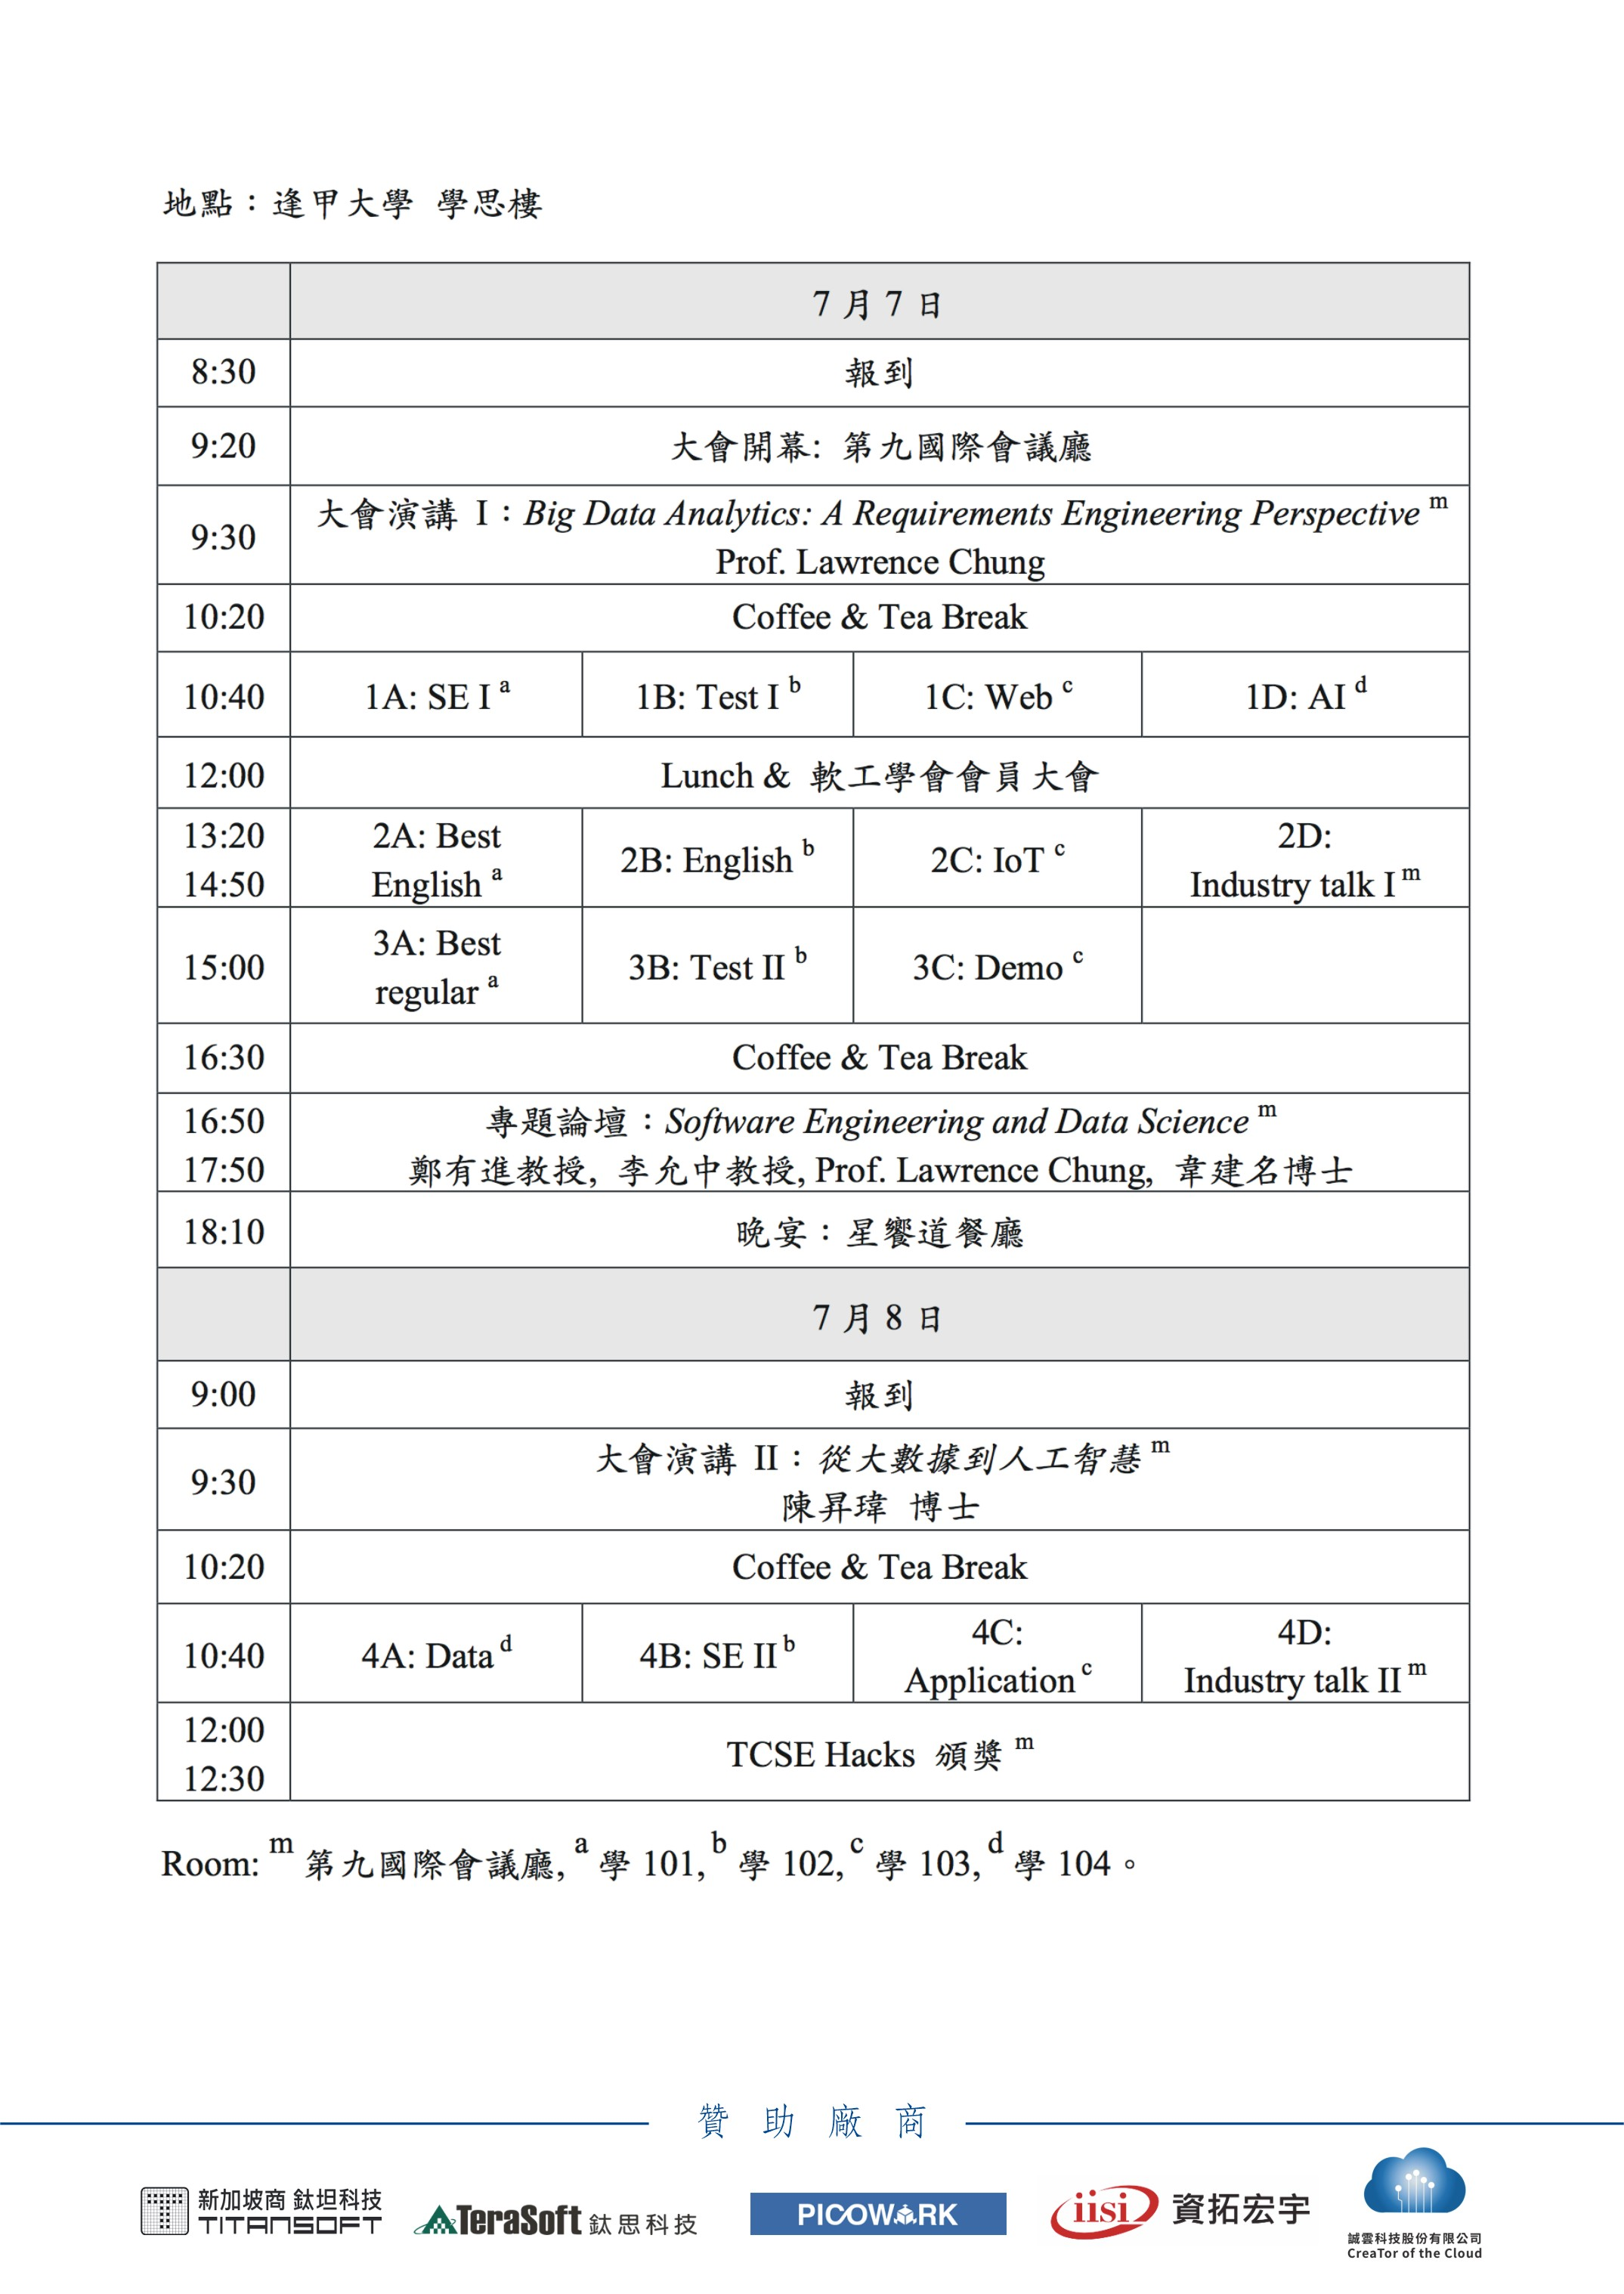
\includepdf[fitpaper]{back} %back page


%\chapter*{會場平面圖}

%\chapter*{接駁車與計程車資訊}

\end{document} 
